\documentclass[12pt]{article}

\usepackage[ansinew]{inputenc}
\usepackage{amsmath}
\usepackage{amsthm}
\usepackage{enumerate}
\usepackage{exscale}
\usepackage{indentfirst}
\usepackage{latexsym}
\usepackage[noend]{algorithmic}
\usepackage{algorithm}
\usepackage{tikz} 
\usepackage{rotating}
\usepackage{hyperref}
\usepackage{color}

\usetikzlibrary{backgrounds,fit,arrows} 

% Page size
\addtolength{\textheight}{2cm}

% Versioning
\newenvironment{nuevo}{\marginpar{$<$nuevo$>$}}{\marginpar{$<$/nuevo$>$}}

% LPs
\newenvironment{lpmodel}{\subsubsection*{Model:} }{ }
\newcommand{\lpobjective}[2]{\textsc{Objective:} #1 \[ #2 \]}
\newcommand{\lprestriction}[3]{\textsc{Subject to:} #1 \[ #2 \qquad #3 \]}

% Acronyms
\newcommand{\PCP}{\textsc{pcp}}
\newcommand{\TODO}[1]{\textcolor{red}{[\textbf{\textsc{ToDo:} #1}]}}

% Items
\newcommand{\defitem}[2]{\item{\textbf{#1:} #2}}

% Math
\newcommand{\sumheight}{\ensuremath{\phantom{\sum_{j \in C}}}}
\newcommand{\ceil}[1]{\ensuremath{\left\lceil #1 \right\rceil}}
\newcommand{\floor}[1]{\ensuremath{\left\lfloor #1 \right\rfloor}}

% Algorithmics
\newcommand{\algorithmiccall}{\textbf{call}\ }
\newcommand{\algorithmicprocedure}{\textbf{procedure}\ }
\newcommand{\algorithmicendprocedure}{\algorithmicend\ \algorithmicprocedure}
\newenvironment{ALC@proc}{\begin{ALC@g}}{\end{ALC@g}}
\newcommand{\PROC}[1]{\algorithmicprocedure #1\ \begin{ALC@proc}}
\newcommand{\CALL}[1]{\STATE \algorithmiccall #1}
\ifthenelse{\boolean{ALC@noend}}
	{\newcommand{\ENDPROC}{\end{ALC@proc}}}
	{\newcommand{\ENDPROC}{\end{ALC@proc}\ALC@it\algorithmicendprocedure}}

% Configs
\newtheorem{theorem}{Theorem}
\numberwithin{equation}{section}
\numberwithin{table}{section}
\numberwithin{algorithm}{section}

\includeonly{ineqs}

% Document start
\begin{document}

\tableofcontents
\clearpage

%!TEX root = pcp.tex

\section{Introduction}
\label{sec:introduction}

\subsection{Coloring}

Needless to say, graphs are widely used for modeling different scenarios in multiple areas of expertise, as well as for solving problems on those scenarios by translating them into well-known problems. 

One of those problems is the graph coloring problem, which consists in assigning a color to each node in a graph, with the constraint that two adjacent nodes must not have the same color. The objective is to generate a valid coloring using the minimum number of colors.

One of the most famous real life problems which led to the graph coloring problem was the \textit{4 colors problem}. In 1852, the question of whether any planar map could be colored using only four colors, in such a way that no two regions sharing a border had the same color, was posed. Modeling neighbour regions as adjacent nodes in a planar graph led to the planar graph coloring problem, which was eventually generalized into coloring a generic graph.

Graph coloring is widely used in multiple applications, such as schedule assignment to solve time incompatibilities, assignment of radio frequencies to prevent interference between neighboring radios, or even assigning variables to registers during the flow of a program.

The coloring of a graph is defined formally as a function that, given an input graph $G = <V,E>$, being $V$ the set of nodes and $E$ the set of undirected edges, assigns each node $v \in V$ to a natural number which represents a color, such that no two adjacent nodes have the same color. A \textit{k-coloring} is an assignment which uses exactly $k$ different colors.

\begin{figure}[h]
	\centering
	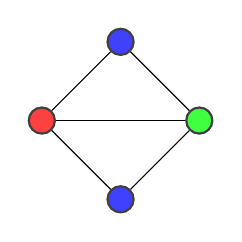
\begin{tikzpicture} 
		[n/.style= {minimum size=3mm,thick,circle,draw=black!75}] 
		
		\node[n,fill=red!75] (n0) at ( 0,0) {}; 
		
		\node[n,fill=blue!75] (n1) at ( 1,1) {}
			edge [-]	(n0)
		;

		\node[n,fill=green!75] (n2) at ( 2,0) {}
			edge [-]	(n1)
			edge [-]	(n0)
		;

		\node[n,fill=blue!75] (n3) at ( 1,-1) {}
			edge [-]	(n2)
			edge [-]	(n0)
		;
		
	\end{tikzpicture} 
\caption{Sample 3-coloring of a diamond graph.}
	\label{fig:samplecoloring}
\end{figure}

This problem has been proved to be \textit{NP-Complete}, and has been widely studied in the literature, being approached both by heuristic and exact methods for its resolution.

\subsubsection*{Previous Work}

Simplest heuristic approaches consist in greedy algorithms, using different criteria such as \textit{largest-first} \cite{welsh1967upper}, \textit{smallest-last} \cite{matula1972graph} or \textit{degree of saturation} \cite{brelaz1979new}. While the first two rely on a static ordering based on the degree of each node, the last one uses a dynamic ordering based on the number of different colors being used in the neighbourhood of each vertex.

These criteria may also be used in implicit enumeration techniques, which enumerate the possible colorings in the order determined by the chosen criteria. Using a good strategy is vital for finding good solutions as soon as possible, therefore pruning a great number of colorings. The implicit solution tree may be traversed in a BFS, DFS or best bound fashion. All these algorithms eventually find the optimal solution for the problem.

The \textsc{dsatur} enumeration algorithm proposed in \cite{brelaz1979new} has proven to be one of the most efficient implicit enumeration methods for the coloring problem, having several improvements such as \cite{sewell1996improved}.

More complex heuristic algorithms, using different metaheuristics, have also been used for the coloring problem.

There is also extensive work using integer linear programming formulations for the coloring problem by using different models:
\begin{itemize}
\item{In \cite{mehrotra1996column} a column generation approach is used based on an independent set formulation of the problem, in which a binary variable $x_S$ defines whether the independent set $S$ is given a color label or not; this formulation requires a variable for each possible color class in the graph.}
\item{An ILP model for acyclic orientations with path constraints is presented in \cite{figueiredo2005acyclic} and then applied to solve the vertex coloring problem.}
\item{The representatives model presented in \cite{campelo2004cliques} and \cite{campelo2008asymmetric} uses $x_{uv}$ variables which determine whether vertex $v$ \textit{represents} color $u$; having exactly one node represent each color class allows easy symmetry breaking.}
\item{In \cite{mendez2006branch,mendez2008cutting} both branch-and-cut and cutting planes algorithms were developed for a standard formulation of the problem, using $x_{ij}$ variables to specify whether node $i$ used color $j$, and $w_j$ variables as witnesses to whether color $j$ was in use. Several symmetry breaking constraints were added to the model to ensure a fast resolution.}
\end{itemize}

\subsection{Routing and Wavelength Assignment in WDM Networks}

A Wavelength Division Multiplexed (WDM) optical network consists in a network in which links are optical fibers capable of transmitting a specified number of different wavelengths. The Routing and Wavelength Assignment (RWA) problem consists in, given a desired set of connections between pairs of nodes, establish routes between those nodes using the network's links.

Every route is composed by a set of consecutive lightpaths. A lightpath is defined as a point to point connection between two adjacent nodes in the network using a certain wavelength. Although there are networks in which the nodes are capable of transforming wavelengths within the same route, we will assume that every route uses the same wavelength across all of its lightpaths; this restriction is known as the \textit{wavelength continuity constraint}.

The second restriction to be satisfied is the \textit{wavelength clash constraint} which imposes that different lightpaths in the same physical link must have different wavelengths. Together with the previous constraint, it is implied that two different routes that share at least one physical link must use different wavelengths.

In the offline or static version of the RWA problem, the set of connections to be established is known beforehand. The counterpart of this version is the \textit{dynamic} RWA in which connections must be satisfied as they are requested in an online fashion. In this work we will take only the former version into consideration.

The goal of the min-RWA is to minimize the number of different wavelengths required to establish all the routes desired. Note that there are multiple criteria that can be used to evaluate the quality of a set of routes, such as the number of lightpaths used for each route, or generating particular traffic patterns. In this work we will be focusing only in optimizing the number of wavelengths.

\subsection*{Previous Work}

Initial techniques to solve the min-RWA problem as a two-stage problem, such as \cite{hyytia14wavelength}, pick a single route for every connection using shortest-path algorithms and then use different heuristics to solve a standard coloring problem in the assignment stage. In \cite{manohar2002routing} the shortest-path routing solution is replaced by a maximum edge disjoint path solution in order to reduce conflicts between routes.

Other approaches to the problem tackle the routing and wavelength assignment as a single problem, without decomposing it in two separate phases. In \cite{skorin2007routing}, for example, bin packing heuristic algorithms are used to handle the problem, whereas \cite{noronha2007random} embeds this heuristic into a genetic evolutionary framework.

An exact approach using an integer programming formulation with column generation is used in \cite{lee2002optimization}, which solves both the routing and the wavelength assignment problems in the same formulation.

\subsection{Partitioned graph coloring problem}

A \textit{partitioned graph} is defined as a tuple $G = <V,E,P>$ of $n$ vertices, $m$ edges and $q$ partitions respectively. The set $P$ contains $P_1, \ldots ,P_q$ sets of nodes which constitute a partition of $V$. Therefore, for every node $v \in V$, there is exactly one $P_k \in P$ such that $v \in P_k$, and every $P_i \in P$ is nonempty.

The partitioned coloring problem is defined as an assignment of colors to the nodes of the graph $G$, with the restriction that no two adjacent nodes may have the same color, but requiring only one node per partition to be colored. Once again, the goal is to minimize the number of colors required.

\begin{figure}[h]
	\centering
	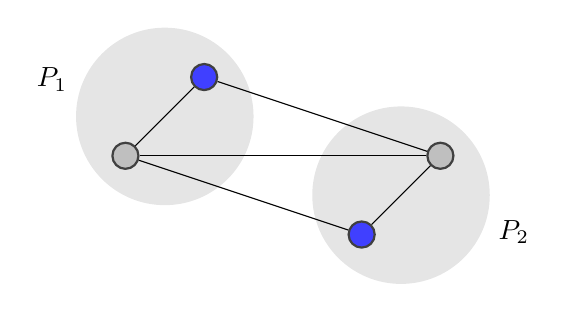
\begin{tikzpicture} 
		[n/.style= {minimum size=3mm,thick,circle,draw=black!75}] 
		
		\node[n,fill=black!25] (n0) at ( 0,0) {}; 
		
		\node[n,fill=blue!75] (n1) at ( 1,1) {}
			edge [-]	(n0)
		;

		\node[n,fill=black!25] (n2) at ( 4,0) {}
			edge [-]	(n1)
			edge [-]	(n0)
		;

		\node[n,fill=blue!75] (n3) at ( 3,-1) {}
			edge [-]	(n2)
			edge [-]	(n0)
		;
		
			\begin{pgfonlayer}{background} 
				\node [fill=black!10,circle,fit=(n0) (n1),label=170:$P_1$] {}; 
				\node [fill=black!10,circle,fit=(n2) (n3),label=350:$P_2$] {}; 
			\end{pgfonlayer}
		
	\end{tikzpicture} 
\caption{Sample 1-coloring of a partitioned diamond graph.}
	\label{fig:samplepartitionedcoloring}
\end{figure}

\subsubsection*{Complexity}

It is easy to see that when $|P_i| = 1\ \forall P_i \in P$, this is, there is a single node per partition, the partitioned coloring problem is equivalent to the standard graph coloring problem previously mentioned. In terms of complexity classes, PCP belongs to the same class as the standard coloring problem.

\begin{theorem}
The decision version of PCP is NP-Complete.
\end{theorem}

\begin{proof}
We will prove NP-Completeness by proving both belonging to NP and NP-Hard classes.

\begin{itemize}
\item{\textit{NP:} Given an input partitioned graph $G = <V,E,P>$ and an assignment of colors for a subset of nodes, checking that the number of colors used is $k$ is trivial, and a simple algorithm such as \ref{alg:pcpvalidity} can easily check the validity of the coloring in polynomial time.}
\item{\textit{NP-Hard:} Any instance of standard graph $k-coloring$ can be converted to an instance of PCP by partitioning the initial graph $G$ in such a way that every partition contains a single node. The solution to the original $k-coloring$ problem is the same as the solution to the constructed \PCP{}. Since standard coloring is NP-Hard, this implies that PCP is NP-Hard as well.}
\end{itemize}

\end{proof}

\begin{algorithm}
\caption{Polynomial time algorithm for checking validity of a partition coloring}
\label{alg:pcpvalidity}
\begin{algorithmic}

\FORALL{partition $p$ in $P$}
	\FORALL{node $v$ in $p$}
		\IF {$v$ has a color $j$ assigned}
			\STATE mark $p$ as colored
			\FORALL {neighbour $u$ to $v$}
				\IF{$u$ has the same color assigned as $v$}
					\RETURN false
				\ENDIF	
			\ENDFOR
		\ENDIF
	\ENDFOR
	\IF {no node $v$ in $P$ was colored}	
		\RETURN false
	\ENDIF	
\ENDFOR

\end{algorithmic}
\end{algorithm}

\subsubsection*{Resolution of min-RWA using PCP}

There are multiple methods, both heuristic and exact, for solving the min-RWA problem. Some of them handle both the routing and the wavelength assignment as the same problem, whereas other methods, such as the one proposed in \cite{Li00thepartition}, use a two-phase approach: a routing phase and an assignment phase.

In the routing phase, a set of potential routes is generated for every pair of nodes to be connected, mostly using shortest-path criteria.

The assignment phase then requires to pick a route from the set of candidates for every connection. The route chosen is assigned a wavelength, in such a way that no pair of routes that share a physical link have the same wavelength. This phase can be transformed into an instance of \PCP{}.

A partitioned graph $G$ can be constructed in the following way:
\begin{itemize}
\item{Every potential route generated in the routing phase is represented by a node $v \in V$.}
\item{Nodes belong to the same partition iff the routes they represent satisfy the same connection request.}
\item{An edge between two nodes $u,v$ is created if the routes share any physical link.}
\end{itemize}

\begin{figure}[h]
	
	\centering
	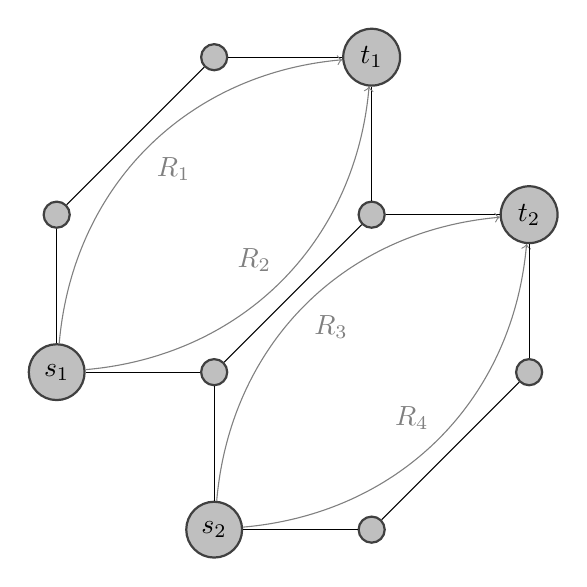
\begin{tikzpicture} 
		[bend angle=40,
		n/.style= {minimum size=3mm,thick,circle,draw=black!75,fill=black!25}] 
		
		\node[n] (n0) at ( 0,0) {$s_1$}; 
		
		\node[n] (n1) at ( 0,2) {}
			edge [-]	(n0)
		;

		\node[n] (n2) at ( 2,4) {}
			edge [-]	(n1)
		;
		
		\node[n] (n4) at ( 2,0) {}
			edge [-]	(n0)
		;
		
		\node[n] (n5) at ( 4,2) {}
			edge [-]	(n4)
		;
		
		\node[n] (n3) at ( 4,4) {$t_1$}
			edge [-]	(n2)
			edge [-]	(n5)
			edge [<-, bend right, draw=black!50] node[auto] {\textcolor{black!50}{$R_1$}} 	(n0)
			edge [<-, bend left, draw=black!50] node[auto,swap] {\textcolor{black!50}{$R_2$}} (n0)
		;
		
		\node[n] (n6) at ( 2,-2) {$s_2$}
			edge [-]	(n4)
		;
		
		\node[n] (n7) at ( 6,2) {$t_2$}
			edge [-]	(n5)
			edge [<-, bend right, draw=black!50] node[auto] {\textcolor{black!50}{$R_3$}}  (n6)
			edge [<-, bend left, draw=black!50]	node[auto,swap] {\textcolor{black!50}{$R_4$}} (n6) 
		;
		
		\node[n] (n8) at ( 4,-2) {}
			edge [-]	(n6)
		;

		\node[n] (n9) at ( 6,0) {}
			edge [-]	(n8)
			edge [-]	(n7)
		;
		
	\end{tikzpicture} 

		\caption{Sample network in which connections $s_1 \rightarrow t_1$ and $s_2 \rightarrow t_2$ are to be implemented. Potential routes $R_1, R_2$ are proposed for the first, while routes $R_3, R_4$ are proposed for the second one. The corresponding partitioned graph is presented in figure \ref{fig:solvedsamplerouting}.}
		
		\label{fig:samplerouting}
	\end{figure}
	
\begin{figure}[h]

		\centering	
		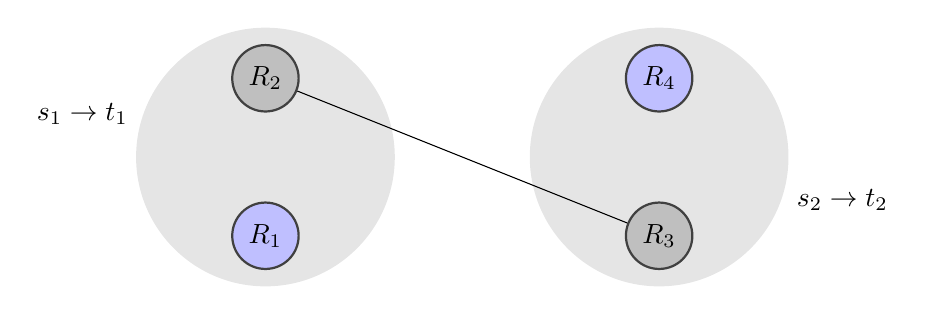
\begin{tikzpicture} 
			[n/.style= {minimum size=3mm,thick,circle,draw=black!75}] 

			\node[n,fill=blue!25] (n0) at ( 0,0) {$R_1$}; 

			\node[n,fill=black!25] (n1) at ( 0,2) {$R_2$};

			\node[n,fill=black!25] (n2) at ( 5,0) {$R_3$}
				edge [-]	(n1)
			;

			\node[n,fill=blue!25] (n3) at ( 5,2) {$R_4$};

				\begin{pgfonlayer}{background} 
					\node [fill=black!10,circle,fit=(n0) (n1),label=170:$s_1 \rightarrow t_1$] {}; 
					\node [fill=black!10,circle,fit=(n2) (n3),label=350:$s_2 \rightarrow t_2$] {}; 
				\end{pgfonlayer}

		\end{tikzpicture} 
	
		\caption{Conflicts partitioned graph for network from figure \ref{fig:samplerouting}. Routes $R_1$ and $R_2$ satisfy the same connection request, as such, they are contained in the same partition; same happens for $R_3$ and $R_4$. Since routes $R_2$ and $R_3$ share a physical link, the corresponding nodes are adjacent to prevent that they are assigned the same frequency. A 1-coloring, which assigns the same label to $R_1$ and $R_4$ is shown, and the corresponding lightpaths generated are shown in figure \ref{fig:solvedsampleroutingnetwork}.}

		\label{fig:solvedsamplerouting}
\end{figure}

\begin{figure}[h]
	\centering
	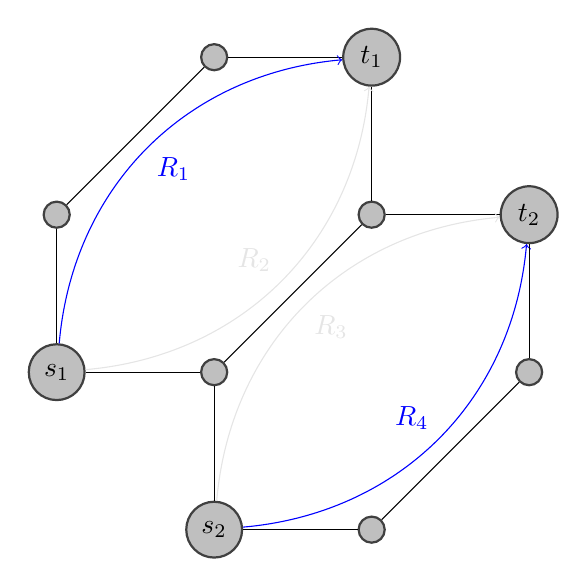
\begin{tikzpicture} 
		[bend angle=40,
		n/.style= {minimum size=3mm,thick,circle,draw=black!75,fill=black!25}] 
		
		\node[n] (n0) at ( 0,0) {$s_1$}; 
		
		\node[n] (n1) at ( 0,2) {}
			edge [-]	(n0)
		;

		\node[n] (n2) at ( 2,4) {}
			edge [-]	(n1)
		;
		
		\node[n] (n4) at ( 2,0) {}
			edge [-]	(n0)
		;
		
		\node[n] (n5) at ( 4,2) {}
			edge [-]	(n4)
		;
		
		\node[n] (n3) at ( 4,4) {$t_1$}
			edge [-]	(n2)
			edge [-]	(n5)
			edge [<-, bend right, draw=blue!100] node[auto] {\textcolor{blue!100}{$R_1$}} 	(n0)
			edge [<-, bend left, draw=black!10] node[auto,swap] {\textcolor{black!10}{$R_2$}} (n0)
		;
		
		\node[n] (n6) at ( 2,-2) {$s_2$}
			edge [-]	(n4)
		;
		
		\node[n] (n7) at ( 6,2) {$t_2$}
			edge [-]	(n5)
			edge [<-, bend right, draw=black!10] node[auto] {\textcolor{black!10}{$R_3$}}  (n6)
			edge [<-, bend left, draw=blue!100]	node[auto,swap] {\textcolor{blue!100}{$R_4$}} (n6) 
		;
		
		\node[n] (n8) at ( 4,-2) {}
			edge [-]	(n6)
		;

		\node[n] (n9) at ( 6,0) {}
			edge [-]	(n8)
			edge [-]	(n7)
		;
		
	\end{tikzpicture} 
		
		\caption{Solution for the network presented in figure \ref{fig:samplerouting} using the coloring obtained in \ref{fig:solvedsamplerouting}. Since $R_1$ and $R_4$ were the colored nodes, using the same label, then those are the routes established and lightpaths using that label are created to satisfy the connection requests.}
		\label{fig:solvedsampleroutingnetwork}
	\end{figure}

Each wavelength is represented as a color. The problem then consists in coloring a single node within each partition, this is, assigning a wavelength to a single route from the set of candidates for each connection request. The fact that two nodes may not be colored if they are adjacent guarantees  that no wavelength conflicts may occur between two different lightpaths in the same link.

An example is shown in figures \ref{fig:samplerouting}, \ref{fig:solvedsamplerouting} and \ref{fig:solvedsampleroutingnetwork}.

In this work we will focus on finding an exact solution for the partitioned coloring problem, using a branch and cut algorithm based on a generalization of the coloring model proposed in \cite{mendez2006branch,mendez2008cutting}.

\subsubsection*{Previous work}

In \cite{Li00thepartition}, two groups of heuristics were developed for solving the \PCP{}: one-step and two-step. The former consists in picking the easiest node to color in every partition, and then picking the hardest one from that set using different criteria (largest-first, smallest-last, color-degree); the latter makes an initial pass picking the easiest nodes in every partition and inducing a non-partitioned graph, onto which a standard heuristic is applied in a second stage.

In \cite{noronha2006routing} the one-step color-degree constructive heuristic is used in a tabu search approach, TS-PCP. Routes are generated in an initial stage using a $k$-EDR constructive procedure, based on the maximum edge disjoint path heuristic by \cite{kleinberg1996approximation}, and the resulting partitioned coloring problem is solved with TS-PCP.

Due to the complexity of the problem, most of the work on PCP is composed by heuristic approaches. However, in \cite{frota2010branch}, a branch and cut algorithm is devised, using an integer linear programming model based on the asymmetric representatives formulation for the standard coloring problem, presented in \cite{campelo2004cliques} and \cite{campelo2008asymmetric}.

\subsection{Objective of this work}

A common approach for obtaining exact solutions to complex combinatorial optimization problems is to model them as integer linear programming problems, and solve them using branch and bound, cutting planes or branch and cut algorithms, among others. 

Therefore, the objective of this work will be to develop a branch and cut algorithm for solving the partitioned coloring problem, by modelling it as an integer linear programming problem, with a generalization of the standard coloring model presented in \cite{mendez2006branch,mendez2008cutting}. 

We will be using \textsc{cplex} as a branch and cut framework and introduce custom initial heuristics, cutting planes, primal heuristics and branching strategies, designed specifically for this problem, and evaluate their performance against the default implementation provided by \textsc{cplex}.

This work is structured in seven chapters. In chapter \ref{sec:model} we present different models for representing an instance of \PCP{}, starting with a basic model that captures all necessary restrictions, for later strengthening it by modifying the constraints with stronger ones or introducing new ones, such as symmetry breaking constraints.

Chapter \ref{sec:ineqs} dwelves deeper into the polyhedron defined in the previous chapter by presenting valid inequalities derived for \PCP{}. These inequalities will be later applied as cutting planes in both cutting planes and branch and cut algorithms.

Alternative algorithms for solving the problem are presented in chapter \ref{sec:heur}. We present enumeration algorithms for solving the standard coloring problem, and generalize them for partition coloring, focusing in the \textsc{dsatur} algorithm \cite{brelaz1979new} and its generalization. These algorithms will be adapted to be used as initial and primal heuristics during the branch and cut process.

The implemented branch and cut algorithm is presented in chapter \ref{sec:bnc}, where we present the general structure for cutting plane, branch and bound and branch and cut algorithms, as well as different components of a branch and cut (separation heuristics, initial heuristics, primal heuristics, branching strategies, node selection strategies) and how we implemented them for dealing with the \PCP{}.

This implementation is then tested in chapter \ref{sec:results}. Given a test suite of binomial, powerlaw cluster and \textsc{dimacs} challange graphs, we first evaluated multiple configurations for all of the different components, starting by choosing a model to be used in the algorithm, and testing the effectiveness of the different heuristics and strategies with different parameterizations. We then test the performance of the algorithm, once we have all parameters fixed, against a fresh test suite and report the obtained MIP gap.

Finally, in chapter \ref{sec:conclusions}, we sum up the work achieved, draw conclusions from it and present possible future research lines.

\subsection{Definitions}
\label{subsec:intro:definitions}

In this section we will define all concepts and conventions to be used throughout this work: 

\begin{itemize}
	\defitem{Colors}{The set of valid color labels $C = \{1, \ldots, c\}$, where $c$ may be any upper bound to the chromatic number of the graph, such as $n$.}
	\defitem{Graph}{Defined as tuple $<V,E>$ where $V$ is the set containing the $n$ nodes and $E$ contains the $m$ undirected edges.}
	\defitem{Partitioned Graph}{Defined as tuple $<V,E,P>$, being $V$ and $E$ the same sets as above, and $P$ the set of $P_1, \ldots, P_q$ partitions of $V$.}
	\defitem{Partition function}{For every node $v$ in a partitioned graph, $p(v)$ returns the partition that contains that node.}
	\defitem{Neighbourhood}{$N(v)$ is the set of nodes in $V$ adjacent to node $v$.}
	\defitem{Partition Neighbourhood}{$N_P(v)$ is the set of partitions that contain at least one node adjacent to $v$.}
	\defitem{Degree}{$\delta(v)$ is the cardinal of the neighbourhood of $v$.}
	\defitem{Partition Degree}{$\delta_P(v)$ is the cardinal of the partition neighbourhood of $v$.}
	\defitem{Color Degree}{Number of different colors used in $N(v)$ for a node $v \in V$; also degree of saturation.}
	\defitem{Extended Clique}{Subset of $V$ such that for every pair of nodes $u,v$, either $u$ is adjacent to $v$ or $u$ and $v$ are contained in the same partition.}
	\defitem{Component Independent Set}{Subset of $V$ such that for every pair of nodes $u,v$, $u$ is not adjacent to $v$ and they belong to different partitions.}
	\defitem{Partition Graph}{The \textit{partition graph} $G'$ of a partitioned graph $G$ is a standard graph $G'=<V',E'>$ in which every node $v'_k \in V'$ corresponds to a partition $P_k \in P$, and two nodes $v'_i,v'_j \in V'$ are adjacent if and only if every node in $P_i$ in $G$ is adjacent to every node in $P_j$.}
\end{itemize}

%!TEX root = pcp.tex

\section{Model}
\label{sec:model}

In this section we will present the BIP formulation for the \PCP{}, as a generalization of the CP model used by M\'endez-D\'iaz and Zabala in \cite{mendez2008cutting}.

\subsection{Formulation}
\label{subsec:model:formulation}

Let $G = <V,E,P>$ a partitioned graph, being $V$ the set of nodes numbered from $1$ to $n$, $E$ the set of $m$ edges, and $P$ the set of partitions numbered from $1$ to $q$; and let $C$ be the set of color labels numbered from $1$ to $n$.

The standard coloring problem formulation, SCP, uses the following $(n + 1) \times c$ binary variables, where $i \in V$ and $j \in C$:
\begin{itemize}
\item $x_{ij}$ equals $1$ if and only if the node $i$ is colored with label $j$
\item $w_j$ equals $1$ if there is at least one node in the graph which uses color $j$
\end{itemize}

The goal is to minimize the total number of colors used, this is, the number of $w_j$ variables set to $1$.

\begin{align}
\text{\textsc{minimize}} \quad & \sum_{j \in C} w_j \nonumber \\
\text{\textsc{subject to}} \quad & \sum_{j \in C} x_{ij} = 1 \quad \forall i \in V \label{eqn:vertexsum} \\
& x_{ij} + x_{kj} \leq w_j \quad \forall (i,k) \in E, \; \forall j \in C \sumheight \label{eqn:adjscolor}\\
& x_{ij}, w_{j} \in \{0,1\} \quad \forall i \in V, \; \forall j \in C \sumheight \nonumber
\end{align}

Equation \ref{eqn:adjscolor} implies that two adjacent vertices may not use the same color, and also ensures that any variable $x_{ij}$ set to $1$ will cause $w_j$ to be set as well.

Restriction \ref{eqn:vertexsum} requires that every node is assigned exactly one color. Since the difference between standard coloring and partition coloring relies solely in the fact that, in the latter, only one node per partition must be colored, adjusting this last restriction provides a simple model for PCP.

\begin{align}
\text{\textsc{minimize}} \quad & \sum_{j \in C} w_j \label{eqn:obj} \\
\text{\textsc{subject to}} \quad & \sum_{i \in P_k} \sum_{j \in C} x_{ij} = 1 \quad \forall P_k \in P \label{eqn:partsum} \\
& x_{ij} + x_{kj} \leq w_j \quad \forall (i,k) \in E, \; \forall j \in C \sumheight \label{eqn:adjscolorp}\\
& x_{ij}, w_{j} \in \{0,1\} \quad \forall i \in V, \; \forall j \in C \sumheight \nonumber
\end{align}

This model has $(n + 1) \times c$ variables as well, $q$ restrictions \ref{eqn:partsum} and $m \times c$ \ref{eqn:adjscolorp} restrictions, plus all integrality constraints.

\subsection{Variants}

There are several variants for the previously presented model for \PCP{}, all of which provide valid partition colorings. We will explore different alternatives to the basic formulation (\ref{eqn:obj},\ref{eqn:partsum},\ref{eqn:adjscolorp}).

\subsubsection{Color a single node per partition}

Restriction \ref{eqn:partsum} can be relaxed by requiring that at least one node is colored per partition, instead of requiring that exactly one node is colored. Even more, we may also accept colorings in which a single node is assigned more than one color. 

\begin{equation}
\label{eqn:partsumgeq}
\sum_{i \in P_k} \sum_{j \in C} x_{ij} \geq 1
\end{equation}

The minimization of the total number of colors used will ensure that no additional colors will be used, and a valid coloring can be extracted from the resulting solution by picking any color from any node on every partition, as no color conflicts will occur since restriction \ref{eqn:adjscolorp} is still in place.

\subsubsection{Color conflicts}

An alternative to restriction \ref{eqn:adjscolorp}, for both preventing color conflicts and set $w_j$ variables upon usage of color $j$, is to decouple this two concepts into different restrictions. Therefore, instead of restricting $x_{ij} + x_{kj} \leq w_j$ for every edge, we may require:

\begin{align}
x_{ij} + x_{kj} \leq 1 \quad &\forall (i,k) \in E, \; \forall j \in C \label{eqn:adjscolorpone}\\
x_{ij} \leq w_{j} \quad &\forall i \in V, \; \forall j \in C \label{eqn:nodelessthanwj}
\end{align}

This alternative, however, yields an even larger number of restrictions than the original \ref{eqn:adjscolorp}. Looking forward to reducing the number of equations in the model, we propose the following alternative:

\begin{equation}
\label{eqn:adjsperpart}
\sum_{i \in P_k \cap N(i_0)} x_{ij} + x_{i_0j} \leq w_j \quad \forall j \in C, \; \forall P_k \in P, \; \forall i_0 \in V 
\end{equation}

This equation establishes that either node $i_0$ may use color $j$, or at most one neighbor in every adjacent partition may use it (as no more than a single node may be colored per partition). This formulation considerably reduces the amount of restrictions when partition sizes are large; otherwise, it does not report any benefits over the original version \ref{eqn:adjscolorp}.

Another variant that further reduces the number of restrictions makes heavy use of the maximum number of nodes that may use the same color within a neighbourhood:

\begin{equation}
\label{eqn:adjsneighb}
\sum_{i \in N(i_0)} x_{i_0j} + r * x_{i_0j} \leq r * w_j \quad \forall j \in C, \; \forall i_0 \in V 
\end{equation}

A simple value for $r$ could be the number of different partitions in the neighbourhood of node $i_0$. In that case, the restriction implies that either node $i_0$ uses color $j$, or at most $r$ nodes in its neighbourhood may use it simultaneously.

However, we may tighten the restriction by replacing $r$ by the number of components in an extended clique coverage of the node's neighbourhood, as this value provides an upper bound for the maximum number of colors that can be used for a set of nodes. We use a simple greedy heuristic to generate a standard clique cover of the partition graph induced by the neighbourhood of $i_0$ to obtain the value $r$.

This restriction generates a much lower number of equations in dense graphs, as it requires just $c$ restrictions per node instead of per edge.

\subsection{Breaking symmetry}
\label{subsec:model:symmetry}

One of the main issues with the model presented is that it allows for multiple symmetric solutions; the same happens with the standard coloring model SCP. 

Since it does not matter which color labels are used in the coloring, any $\chi$ colors can be used, resulting in $P(c,\chi)$\footnote{Number of different ordered subsets of size $\chi$ from a set of size $c$, equals to $c! / (c - \chi)!$} different solutions for every equivalent coloring; therefore, introducing additional constraints with the purpose of removing symmetric solutions is expected to produce an improvement in the algorithm, as it greatly limits the solution space.

The easiest restriction to generate is to prevent color $j+1$ from being used unless color $j$ is used in the coloring. This ensures that only colors with labels $1 \ldots k$ are used in a k-coloring, leaving always the last $k+1 \ldots c$ unused, thus reducing the number of symmetric solutions from $P(c,k)$ to $k!$.

\begin{equation}
\label{eqn:lowerlabel}
w_j \geq w_{j+1} \quad \forall 1 \leq j < c 
\end{equation}

A stricter requirement that can be imposed is to forbid having more vertices colored with label $j+1$ than with label $j$. This removes all symmetric solutions in the case that every color class has a different node count, which is a vast improvement from the previous restriction.

\begin{equation}
\label{eqn:symnodecount}
\sum_{i \in V} x_{ij} \geq \sum_{i \in V} x_{ij+1} \quad \forall 1 \leq j < c 
\end{equation}

However, this restriction allows symmetric solutions by exchanging labels between color classes with same cardinal, which is likely to occur in regular graphs. 

In order to completely remove symmetric solutions, it is possible to enforce the following restriction, which implies that among all possible assignments, only the one that assigns the lowest possible color label to the partition with the lowest index is used: 

\begin{align}
x_{ij} = 0 \quad &\forall j > p(i) + 1 \label{eqn:nodeszero} \\
x_{ij} \leq \sum_{l = j-1}^{k-1} \sum_{u \in P_l} x_{uj-1} \quad &\forall 1 < k \leq q, \; \forall i \in P_k, \; \forall 1 < j \leq k \label{eqn:minlabel}
\end{align}

Equation \ref{eqn:nodeszero} establishes that color with label $j$ may not be used for a partition with index greater than $j$; whereas equation \ref{eqn:minlabel} imposes that color $j$ cannot be used for a partition unless color $j-1$ was used in a previous partition.

As an example, suppose a graph such that $P = \{ P_1, \ldots, P_q \}$ and $P_k = \{ x_{2k-1}, x_{2k} \}$, this is, every partition has two nodes. The first instantiations of restriction \ref{eqn:minlabel} would be:

\begin{align*}
k = 2, i = 3, j = 2 \qquad & x_{3,2} \leq \sum_{u \in P_1} x_{u,1} = x_{1,1} + x_{2,1} \\
k = 2, i = 4, j = 2 \qquad & x_{4,2} \leq \sum_{u \in P_1} x_{u,1} = x_{1,1} + x_{2,1} \\
&\\
k = 3, i = 5, j = 2 \qquad & x_{5,2} \leq \sum_{u \in P_1} x_{u,1} + \sum_{u \in P_2} x_{u,1} = x_{1,1} + x_{2,1} + x_{3,1} + x_{4,1} \\
k = 3, i = 6, j = 2 \qquad & x_{6,2} \leq \sum_{u \in P_1} x_{u,1} + \sum_{u \in P_2} x_{u,1} = x_{1,1} + x_{2,1} + x_{3,1} + x_{4,1} \\
&\\
k = 3, i = 5, j = 3 \qquad & x_{5,3} \leq \sum_{u \in P_2} x_{u,2} = x_{3,2} + x_{4,2} \\
k = 3, i = 6, j = 3 \qquad & x_{6,3} \leq \sum_{u \in P_2} x_{u,2} = x_{3,2} + x_{4,2} \\
\vdots \qquad & \vdots
\end{align*}

\subsection{Objective function}
\label{subsec:model:obj}

Another way of reducing the number of symmetric solutions is to prefer lower-label colors in the objective function, therefore choosing the lowest labels possible in each coloring. To achieve this we simply add higher coefficients to lower $w_j$ variables in the objective:

\begin{equation}
\label{eqn:objlinear}
\text{\textsc{minimize}} \quad \sum_{j \in C} j \times w_j 
\end{equation}

However, early tests showed that this objective function offers poor computational results, so it was early discarded from the set of possible formulations.

\subsection{Strengthening the model}

There are other inequalities, besides the already mentioned symmetry breaking ones, that are not necessary for the formulation of a valid coloring, yet they strengthen the model relaxation, helping during the branch and cut process. These inequalities are entirely optional in the formulation, their inclusion depends strictly in the tradeoff between building a more complex model that takes more time to solve and strengthening its relaxation so the algorithm's overall performance is increased.

A simple restriction, which is already implied by the objective function, consists in preventing a $w_j$ variable from being set unless there is a node painted with color $j$:

\begin{equation}
\label{eqn:wjleqsumcolor}
w_j \leq \sum_{i \in V} x_{ij} \quad \forall j \in C
\end{equation}

The usage of this restriction will become clear when we present the branching strategies in \ref{subsec:alg:branching}, in which we directly enforce bounds on the $w_j$ variables based on additional information on the coloring problem.

Another equation, which improved the obtained results in \cite{mendez2006branch}, avoids the generation of fractional solutions such as $x_{ij} = 1/c$:
\begin{equation}
\label{eqn:wjgeqsumnode}
\sum_{j \in C} w_j \geq \sum_{j \in C} j x_{ij} \quad \forall i \in V
\end{equation}

The rationale behind that restriction is that only one $x_{ij}$ may be set per node, therefore the right hand side of the inequality is the label of the color assigned to node $i$, which cannot be greater than the total of colors used.

This restriction can be further strengthened by extending the sum of the $x_{ij}$ variables over partitions instead of nodes:
\begin{equation}
\label{eqn:wjgeqsumpart}
\sum_{j \in C} w_j \geq \sum_{j \in C} \sum_{i \in P_k} j x_{ij} \quad \forall P_k \in P
\end{equation}


%!TEX root = pcp.tex

\section{Valid inequalities}

In this section we will analyze the PCP polyhedron and derive valid inequalities for it, that will be later used in the branch-and-cut algorithm in cutting planes. We will focus our analysis on the most basic formulation presented in section \ref{subsec:model:formulation}, except for some inequalities which will exploit symmetry breaking restrictions from \ref{subsec:model:symmetry}. 

\begin{align}
\text{\textsc{minimize}} \quad & \sum_{j \in C} w_j \nonumber \\
\text{\textsc{subject to}} \quad & \sum_{i \in P_k} \sum_{j \in C} x_{ij} = 1 \quad \forall P_k \in P \nonumber \\
& x_{ij} + x_{kj} \leq w_j \quad \forall (i,k) \in E, \; \forall j \in C \sumheight \nonumber \\
& x_{ij}, w_{j} \in \{0,1\} \quad \forall i \in V, \; \forall j \in C \sumheight \nonumber
\end{align}

Note that any valid inequalities found for the basic formulation are still valid for any other strengthened models, so the derived inequalities can still be used as cuts regardless of the model implemented.

\subsection{Extended clique inequalities}

A classical inequality for the standard coloring problem is the clique inequality, which establishes that within a clique $K$, at most one node can be colored with a label $j$.

\begin{equation}
\nonumber
\sum_{i \in K} x_{ij} \leq w_{j} \quad \forall j \in C
\end{equation}

Combining this inequality with the fact that in PCP at most one node per partition can be colored with a label $j$, we define the \textit{extended clique inequalities} for PCP. Recall from \ref{subsec:intro:definitions} that an extended clique is a maximal subset $K_P$ of $V$ such that every pair of nodes is either adjacent or belong to the same partition.

\begin{equation}
\label{ineq:extendedclique}
\sum_{i \in K_P} x_{ij} \leq w_{j} \quad \forall j \in C
\end{equation}

Similar inequalities were developed by \cite{frota2010branch}, based on the asymmetric representatives formulation, but are generated only on component cliques\footnote{Clique in which every node belongs to a different partition.}. Extended cliques have the added benefit of covering a larger set of nodes, and maintain their effectiveness regardless of the partition size used.

\subsection{Component independent set inequalities}

As was defined in \ref{subsec:intro:definitions}, a component independent set $I_P$ is a standard independent set with the added restriction that every node must belong to a different partition. This allows to import the independent set inequality directly from the standard coloring problem.

\begin{equation}
\label{ineq:ciset}
\sum _{i \in W} x_{ij} \leq \alpha_P(W) w_{j} \quad \forall j \in C
\end{equation}

The restriction is applied to a subgraph of $G$ induced by the nodes $W \subseteq V$. Since the cardinal of the maximum component independent set of the subgraph, $\alpha_P(W)$, is not easy to calculate, being as difficult as the coloring problem trying to solve, this inequality is applied to particular subsets of the graph with an $\alpha_P$ easy to obtain.

\subsubsection*{Component hole inequalities}

A simple instantiation of the previous inequality is picking a subset $W$ that induces a component hole $H$\footnote{A component hole is a chordless cycle in which every node belongs to a different partition.} in the partitioned graph. As in a standard hole, it holds that $\alpha(H) = \floor{n / 2}$, where $n$ is the length of the hole, therefore the only effort required lies in finding a hole and not in calculating its $\alpha$.

Therefore, given a component hole $H$ in the partitioned graph, the component hole inequality is:

\begin{equation}
\label{ineq:chole}
\sum _{i \in H} x_{ij} \leq \floor{n / 2} w_{j} \quad \forall j \in C
\end{equation}


\subsubsection*{Component path inequalities}

Similar to the previous case, the component independent set can be instantiated with a component path $P$, which is a standard path where every node belongs to a different partition. In this case, it holds that for every component path of length $n$, $\alpha(P) = \ceil{n / 2}$, and the inequality results:

\begin{equation}
\label{ineq:cpath}
\sum _{i \in P} x_{ij} \leq \ceil{n / 2} w_{j} \quad \forall j \in C
\end{equation}

\subsubsection*{Strengthening by breaking symmetry}

Component independent set inequalities can be strengthened by taking into consideration symmetry breaking constraints \ref{eqn:lowerlabel} $w_j \geq w_{j+1}$. In case a component independent of size $\alpha_P$ set is colored with label $j^* \leq q - \alpha_P$, then it is possible to ensure that the colors with the highest label will be left unused, since there are $\alpha_P$ nodes using the same color $j^*$.

Therefore, in the worst case, in which all nodes in $V \setminus W$ use different colors, then an assignment as the one shown in table \ref{table:cisetcoloring} will occur. This coloring uses only the first $q - \alpha_P + 1$ colors, and leaves all colors with a greater label unused. 

\begin{table}
\centering	
\begin{tabular}{cc}
\hline
\textbf{color label} & \textbf{partitions count} \\
\hline
$j_0$ & $1$\\
$j_1$ & $1$\\
\vdots & \vdots \\
$j^*$ & $\alpha_P$ \\
\vdots & \vdots \\
$j_{q - \alpha_P}$ & $1$\\
$j_{q - \alpha_P + 1}$ & $1$\\
$j_{q - \alpha_P + 2}$ & $0$\\
\vdots & \vdots \\
$j_{q}$ & $0$\\
\hline
\end{tabular}
\caption{Worst-case color assignment when a component independent set of size $\alpha_P$ is found in the partitioned graph.}
	\label{table:cisetcoloring}
\end{table}

This assignment may happen only if every node outside the $W$ uses a different color, if there is any node repeating color then label $q - \alpha_P + 1$ is unused as well. Therefore, at most one node may be colored using $q - \alpha_P + 1$, while colors with a greater label will never be used, so the following inequality holds:

\begin{equation}
\label{ineq:cisetbshigh}
\sum ^c _{j = j_t + 1} \sum _{i \in V} x_{ij} \leq w_{j_t + 1} \quad j_t = q - \alpha_P(W)
\end{equation}

Combining this inequality with \ref{ineq:ciset}, results in the following component independent set inequality, strengthened via symmetry breaking:

\begin{equation}
\label{ineq:cisetbs}
\sum_{i \in W} x_{ij_0} + \sum ^c _{j = j_t + 1} \sum _{i \in V} x_{ij} \leq \alpha_P(W) w_{j_0} + w_{j_t + 1} \quad \forall j_0 \leq j_t, \; j_t = q - \alpha_P(W)
\end{equation}

Both component hole (\ref{ineq:chole}) and component path inequalities (\ref{ineq:cpath}) can be strengthened using this argument.

\subsection{Partitions graph inequalities}

Let $G' = <V',E'>$ be the partitions graph of $G$\footnote{The partitions graph $G'$ of a partitioned graph $G$ is a standard graph $G'=<V',E'>$ in which every node $v' \in V'$ corresponds to a partition $P_v \in P$, and two nodes $u',v' \in V'$ are adjacent if and only if every node in $P_u$ in $G$ is adjacent to every node in $P_v$.}. Most bounds found for coloring $G'$ can be ported to the original $G$ by extending the constraint over every node represented by each $p \in V'$.

A clear example are independent set inequalities. Let $W' \subseteq V'$ a subset of nodes inducing a subgraph in $G'$, then the independent set inequality holds:

\begin{equation}
\label{ineq:gpiset}
\sum _{i \in W'} x_{ij} \leq \alpha(W') w_{j} \quad \forall j \in C
\end{equation}

As before, in inequalities \ref{ineq:cisetbs}, this restriction can be strengthened considering symmetry breaking constraints:

\begin{equation}
\label{ineq:gpisetbs}
\sum_{i \in W'} x_{ij_0} + \sum ^c _{j = j_t + 1} \sum _{i \in V'} x_{ij} \leq \alpha(W') w_{j_0} + w_{j_t + 1} \quad \forall j_0 \leq j_t, \; j_t = q - \alpha(W')
\end{equation}

These constraints over $G'$ can be converted to constraints $G$ by replacing every node $p \in V'$ with the sum over the nodes $v \in P_p$. Let $W \subseteq P$ be the set of partitions represented by the nodes in $W' \in V'$ in $G'$, then:

\begin{equation}
\label{ineq:gpisetbsg}
\sum_{P_k \in W} \sum_{i \in P_k} x_{ij_0} + \sum ^c _{j = j_t + 1} \sum _{i \in V} x_{ij} \leq \alpha(W') w_{j_0} + w_{j_t + 1} \quad \forall j_0 \leq j_t, \; j_t = q - \alpha(W')
\end{equation}

Once again, since the size $\alpha$ of the maximum independent set of a graph is NP-hard to calculate, the subgraph induced by $W'$ is chosen in such a way that this number is trivial to obtain. These inequality is therefore specialized when $W'$ induces both a path and a hole in $G'$, having $\alpha(W)$ equal to $\ceil{|W| / 2}$ and $\floor{|W| / 2}$, yielding \textit{partitions graph path inequalities} and \textit{partitions graph hole inequalities}, respectively.

Comparing partitions graph independent set inequalities with component independent set ones, the former are less frequent than the latter, since $G'$ tends to be less dense as partition sizes increase; however, the former are much stronger as they impose restrictions over all the nodes in the partitions covered, instead of over a single node per partition.

\subsection{Block color inequalities}

Block color inequalities arise from the symmetry breaking constraints \ref{eqn:lowerlabel} $w_j \geq w_{j+1}$. Given a partition $P_k$ and a color $j_0$, every coloring of partition $P_k$ using any color $j > j_0$, requires that color $j_0$ is already used, since \ref{eqn:lowerlabel} implies that color $j$ cannot be used unless all previous colors had ben used. 

As only a single $x_{ij}$ is set in every partition, this is, only one node is painted with a single color, the following inequality holds:

\begin{equation}
\label{ineq:blockcp}
\sum_{j \geq j_0} \sum_{i \in P_k} x_{ij} \leq w_{j_0} \quad \forall P_k \in P, j_0 \in C
\end{equation}

These $c \times q$ inequalities are extremely easy to generate and, as will be analyzed further in this work, have proven to greatly improve the cutting planes scheme.


%!TEX root = pcp.tex

\section{Enumeration algorithms}
\label{sec:heur}

Implicit enumeration algorithms walk through all possible colorings for the graph, restricting the solution set as much as possible and pruning non-optimal solutions using known bounds. In this section we will review implicit enumeration techniques for the classical coloring problem and discuss different generalizations for \PCP{}.

\subsection{Classical scheme}

A classical scheme for enumeration algorithms is presented in \ref{alg:enumeration}.

\begin{algorithm}
\caption{Classical coloring implicit enumeration scheme for simple graphs $G = <V,E>$}
\label{alg:enumeration}

\begin{algorithmic}
\CALL color(0,1)

\PROC{color(painted, label)}
	\IF{current coloring is no better than best coloring}
		\STATE prune current solutions subtree
	\ELSIF{\textit{painted} equals to $|V|$}
		\STATE update best coloring with current coloring
	\ELSE
		\STATE pick next uncolored \textit{node} to color		
		\FOR{j = 1 to \textit{label}}
			\IF{can paint \textit{node} with color $j$}
				\STATE assign color $j$ to \textit{node}
				\CALL color(painted+1, label)
				\STATE uncolor \textit{node}
			\ENDIF
		\ENDFOR
		\COMMENT{try coloring \textit{node} with a new label}
		\STATE assign color \textit{label} + 1 to \textit{node}
		\CALL color(painted+1, label+1)
		\STATE uncolor \textit{node}
	\ENDIF
\ENDPROC

\end{algorithmic}
\end{algorithm}

The algorithm picks a node to be colored in each recursive call, attempting to color it with one of the already used labels if possible; it also assigns a fresh color to the node, in order to explore all possible colorings for the graph. Note that several symmetric colorings are left out of the exploration. 

At every iteration, the partial solution is pruned if the coloring is using as many labels as the best coloring found by the algorithm, as this implies that the best solution cannot be improved using the current one.

The strategy used for picking the node to be colored in each recursive call gives place to different algorithms. A very simple strategy is to use the degree of the node, coloring nodes with highest degree first, based on the assumption that difficult nodes should be handled early.

Another algorithm, which is one of the most widely used for the coloring problem, is \textsc{dsatur}\cite{brelaz1979new}. This algorithm always picks the node with the highest degree of saturation\footnote{Number of different colors used in $N(v)$ for a node $v \in V$.}, using different strategies for tie-breaking, such as picking the node with the largest number of uncolored neighbours\cite{sewell1996improved}. It has proved to be one of the best enumeration algorithms available.

For an implementation of the \textsc{dsatur} algorithm, we used the code provided by Trick in \cite{trickdsatur}, which we ported to Java and adapted for partitioned coloring as described in \ref{subsec:heur:enumpcp}.

\subsection{Enumerating partitioned colorings}
\label{subsec:heur:enumpcp}

The previous scheme must be modified in order to generate valid partitioned colorings. A simple modification would be to simply pick a new partition instead of a new node on each recursive call, and iterate over all nodes in the partition using all candidate labels. This modification is presented in algorithm \ref{alg:pcpenumerationwrong}. 

\begin{algorithm}
\caption{Modification of enumeration scheme for partitioned graphs $G = <V,E,P>$, picking partitions on every call}
\label{alg:pcpenumerationwrong}

\begin{algorithmic}
		\STATE pick next uncolored \textit{partition} to color		
		\FORALL{\textit{node} in \textit{partition}}
			\FOR{j = 1 to \textit{label}}
				\IF{can paint \textit{node} with color $j$}
					\STATE assign color $j$ to \textit{node}
					\CALL color(painted+1, label)
					\STATE uncolor \textit{node}
				\ENDIF
			\ENDFOR
			\COMMENT{try coloring \textit{node} with a new label}
			\STATE assign color \textit{label} + 1 to \textit{node}
			\CALL color(painted+1, label+1)
			\STATE uncolor \textit{node}
		\ENDFOR
\end{algorithmic}
\end{algorithm}

However, this modification imposes that all the nodes within the same partition are explored together in the enumeration, regardless of the criteria being used to choose each candidate. For example, if a largest-degree criteria is used, and the remaining partitions (with their nodes' degrees) are $P_1 \{v_1(10),v_2(1)\}$ and $P_2 \{v_3(5)\}$, algorithm \ref{alg:pcpenumerationwrong} would enumerate nodes $v_1, v_2, v_3$ instead of $v_1, v_3, v_2$. This severely hurts the efectiveness of the strategy being used.

Therefore, we propose another modification, presented in algorithm \ref{alg:pcpenumeration}. In this case we use the original enumeration scheme, picking a node from an unpainted partition on every call, but before returning from the procedure we create another branch in which we do not color the chosen node, so that the partition can be later colored using another node.

\begin{algorithm}
\caption{Partitioned coloring implicit enumeration scheme for partitioned graphs $G = <V,E,P>$}
\label{alg:pcpenumeration}

\begin{algorithmic}
\CALL color(0,1)

\PROC{color(painted, label)}
	\IF{current coloring is greater than or equal best coloring}
		\STATE prune current solutions subtree
	\ELSIF{\textit{painted} equals to $|P|$}
		\STATE update best coloring with current coloring
	\ELSE
		\STATE pick next uncolored \textit{node} to color	from all uncolored partitions	
		\FOR{j = 1 to \textit{label}}
			\IF{can paint \textit{node} with color $j$}
				\STATE assign color $j$ to \textit{node}
				\CALL color(painted+1, label)
				\STATE uncolor \textit{node}
			\ENDIF
		\ENDFOR
		
		\COMMENT{try coloring \textit{node} with a new label}
		\STATE assign color \textit{label} + 1 to \textit{node}
		\CALL color(painted+1, label+1)
		\STATE uncolor \textit{node}
		
		\COMMENT{leave node unpainted}
		\IF{there are other nodes left in the partition}
			\STATE mark \textit{node} as unavailable
			\CALL color(painted, label)
			\STATE mark \textit{node} as available again
		\ENDIF
		
	\ENDIF
\ENDPROC

\end{algorithmic}
\end{algorithm}

It is within this scheme that we embedded our two different strategies based on degree of saturation for partition coloring.

\subsection{Partitioned \textsc{dsatur}}
\label{subsec:heur:pdsatur}

Classical \textsc{dsatur} picks the node with the highest color degree on each iteration, based on the assumption that nodes difficult to color should be handled first, which usually works well for most heuristics. In the case of partition coloring, as suggested in \cite{Li00thepartition}, nodes with lower degree are easier to color and should be preferred within a partition; also, it is better to color larger partitions first in order to reduce the problem size as early as possible.

Based on these assumptions, we generalized two different versions for partitioned \textsc{dsatur}: \textit{easiest node} and \textit{hardest partition}.

\subsubsection{Easiest node}

The easiest node variant is based on the \textit{onestepCD} heuristic proposed in \cite{Li00thepartition}. In order to pick the node to color, the easiest node is chosen from every uncolored partition, where \textit{easiest} is defined in terms of lowest color degree, with tie breaking on lowest number of uncolored neighbours. From the resulting set, the node with the highest color degree is chosen, as in classic \textsc{dsatur}. 

In other words, this algorithm picks the hardest node from the set of the easiest nodes on each uncolored partition.

Also, in an attempt to explore different solutions earlier to obtain better upper bounds, we also implemented a randomized version of the algorithm. From the set of the easiest nodes in every partition, only half of the time the hardest node is chosen, the other half another candidate is chosen with probability decreasing as its color degree decreases.

\subsubsection{Hardest partition}

Instead of choosing the easiest node from each partition and then picking the hardest one to color, this algorithm first chooses the hardest partition to handle, and then picks the easiest node from that partition. While the easiest node is picked using the usual color degree criteria, choosing the hardest partition requires a new strategy. 

Therefore, in order to determine the hardest partition to color, we experimented with combinations of the following metrics:
\begin{itemize}
	\item{Color degree of the partition, defined as the number of different colors adjacent to all of the nodes in the partition; considering that a larger color degree implies a harder partition to color}
	\item{Size of the partition, as a larger partition being colored earlier helps reducing the problem size, therefore, the larger the partition the earlier it should be handled}
	\item{Number of uncolored partitions adjacent to the partition, equivalent to the tie breaking criteria used for classic \textsc{dsatur}} 
\end{itemize}

Different combinations of these criteria, as well as the different variants of the algorithm, will be compared in section \ref{subsec:resultspdsatur}.

\subsection{Ad-hoc modifications}

As will be presented in section \ref{sec:bnc}, bounded versions of this algorithm will be used during the branch and cut algorithm as an initial heuristic, primal heuristic and subtree pruning. As such, certain adaptations were made to the algorithm.

Since the preprocessing step identifies a large clique before any coloring is performed, the algorithm supports forcing a set of partitions to be assigned a specific set of colors; therefore all partitions $P_{K_1},\ldots,P_{K_\omega}$ contained in the initial clique are colored with labels $1,\ldots,\omega$. The algorithm colors these partitions first, trying all different node combinations within the partitions before proceeding with the partitioned \textsc{dsatur} on the rest of the graph.

Also, since the algorithm is used as a primal heuristic within the branch and cut tree (see \ref{subsec:alg:primal}), it supports forcing the coloring of certain nodes, keeping those assignments fixed during the enumeration process. In case certain node-color combinations are forbidden due to the restrictions imposed during branching, solutions assigning those combinations are not explored in the algorithm.

In case symmetry breaking constraints \ref{eqn:symnodecount} or \ref{eqn:minlabel} are used, the color classes obtained by the algorithm are sorted based on node count or minimum partition index respectively, so the obtained solution can be successfully injected into the branch and cut scheme.



%!TEX root = pcp.tex

\section{Branch and Cut}
\label{sec:bnc}

In this section we will present the implemented branch-and-cut algorithm, including all the components that compose the branch and cut structure, such as initial heuristic, branching strategies, separation algorithms and primal heuristics.

\subsection{Algorithm structure}

The structure of a branch and cut algorithm can be considered a combination of cutting planes and branch and bound schemes, which we describe below.

\subsubsection*{Cutting planes}

Cutting planes algorithms rely solely on valid inequalities for solving the problem. Given a solution of the model's linear relaxation \footnote{The linear relaxation of an integer linear programming consists in removing all integrality constraints on the variables.}, cutting planes are added to the formulation in order to remove the fractional solution obtained. 

Recall that valid inequalities have the property of being satisfied by all integral solutions of the model, but not necessarily by all fractional solutions in the relaxation; therefore, given a fractional solution $x^*$, there is a cutting plane generated by a linear inequality that holds for all integral solution but is not satisfied by $x^*$. 

The algorithm consists in repeating this process, re-solving the relaxation with all added cuts in each iteration, until an integer-feasible solution is obtained.

\begin{algorithm}
\caption{General scheme for a cutting planes algorithm}
\label{alg:cuttingplanes}

\begin{algorithmic}

\LOOP
	\STATE calculate solution of the linear relaxation
	\IF{solution is integral}
		\RETURN obtained solution
	\ENDIF
	\STATE generate a set of cutting planes to cut off the fractional solution
	\STATE add the cutting planes to the model
\ENDLOOP

\end{algorithmic}
\end{algorithm}

The algorithm depends on having an adequate set of cutting planes families, along with good separation heuristics, in order to find valid inequalities that cut off the relaxation's fractional solution on every iteration. Excessive generation of cutting planes may have the drawback that the relaxation becomes larger and larger on every iteration, requiring a greater computational effort to solve.

Note that, besides the valid inequalities specific to each problem, such as the ones we have presented for \PCP{} in section \ref{sec:ineqs}, there are generic families of cutting planes that can be applied to any problem. However, problem-specific cuts usually have better performance than generic ones.

\subsubsection*{Branch and bound}

The branch and bound scheme explores different solutions by setting bounds on fractional variables on every partial solution. The algorithm starts by solving the relaxation, like cutting planes, but instead of removing the fractional solution by adding a valid inequality, it creates two subproblems, usually by fixing a particular variable with a fractional value to either zero or one. 

Each subproblem is then solved using the same strategy until the relaxation's solution is integer feasible, in which case that branch is closed; note that eventually all variables are fixed to an integer value, so an integer solution is always found. The algorithm runs until all nodes are explored.

Besides the \textit{branching} behaviour of the algorithm, both upper and lower \textit{bounds} for each node are considered. A global upper bound (in case of a minimization problem) is updated whenever a new integer feasible solution is found, keeping the one with the lowest objective value. This upper bound is compared with each node's lower bound provided by the relaxation's solution. Since the integer solution will always be greater than the relaxation's, when the lower bound of the node is larger than the global upper bound, the branch can be pruned.

\begin{algorithm}
\caption{General scheme for a branch and bound algorithm}
\label{alg:branchnbound}

\begin{algorithmic}

\STATE initialize \textit{tree} with the problem's formulation
\STATE 
\WHILE{there are open nodes in the \textit{tree}}
	\STATE pick an open \textit{node} from the tree
	\STATE calculate solution $x^*$ of the linear relaxation of the \textit{node}
	\IF{the linear relaxation is infeasible}
		\STATE close the node as the branch is infeasible
	\ELSIF{solution $x^*$ is integer feasible}
		\STATE update best integer solution $x_M$ with $x^*$ if $f(x^*) < f(x_M)$
		\STATE close the node as an integer solution was found
	\ELSIF{$f(x^*) > f(x_M)$} 
		\STATE close the node as best solution cannot be improved
	\ELSE
		\STATE generate new subproblem nodes by \textit{branching}
	\ENDIF
\ENDWHILE

\RETURN best integer solution $x_M$

\end{algorithmic}
\end{algorithm}

The branch and bound scheme does not specify which node to select on each iteration, or how to generate the subproblems on each node. The selection strategy and the branching strategy are chosen depending on the problem to solve.

\subsubsection*{Cut and branch}

The cut and branch scheme is simply an execution of the cutting planes algorithm until a certain threshold is reached (expressed in running time, number of cuts iterations or mip gap). Then the generation of cutting planes is stopped and a branch and bound algorithm is executed, using the initial formulation augmented with all the generated cutting planes.

This algorithm usually yields better results than the previous ones, as cutting planes may have difficulties finding inequalities that remove fractional solutions very close to the convex hull, and a pure branch and bound scheme usually takes too long to solve as the enumeration may be too large. However, since the cutting planes may cause that the relaxations in the branch and bound become tougher to solve, a good balance between the two phases is extremely important for a good overall performance.

\subsubsection*{Branch and cut}

While the cut and branch algorithm applies cutting planes only at the root of the branch and bound tree, the branch and cut version uses cutting planes throughout the whole tree. Although cuts are applied more aggressively at the root, on certain internal nodes more iterations of cuts are executed. 

Note that these generated cuts can use local information, exploiting the variables fixed in the node due to the branching process. In this case, cuts generated on the node are only valid on the node and its subtree; otherwise, cuts generated on an internal node may be reused globally.

An improvement to this scheme consists in deriving integral solutions from node relaxations, obtaining global upper bounds earlier during the traversal, which allow to prune branches earlier. The generation of these solutions is done via \textit{primal heuristics}.

As with all previously mentioned algorithms, branch and cut schemes have a number of parameters and strategies to determine. To begin with, all the separation heuristics for cutting planes iterations must be chosen adequately to quickly find a reasonable number of cuts; on the branch and bound side, node selection and branching strategies must also be determined. Also, the number of cut iterations to perform on the root and on internal nodes must be set, as well as choosing on which nodes cutting planes and primal heuristics should be executed.

Throughout this section we will go over all these missing pieces in the branch and cut structure, and point out how we filled them in the context of the partitioned coloring problem.

\subsection{Preprocessing}

The first step in solving a \PCP{} instance consists in preprocessing the graph, applying all the following rules until no more modifications are made to the graph:

\begin{enumerate}
	\item{As an initial step, every edge with both ends within the same partition is removed. Since only one node is colored per partition, there can be no color conflicts between nodes of the same partition, and all edges connecting them can be removed, in order to greatly reduce the size of the graph and the number of adjacency restrictions generated.}
	\item{Partitions containing isolated nodes can be completely removed from the graph, as any isolated node can be trivially colored using the lowest possible label, and coloring a single node within a partition marks the whole partition as colored, therefore allowing us to completely remove it.}
	\item{Neighbourhood inclusion criteria is applied within a single partition in order to remove higher-order nodes. Let $u,v$ be two different nodes in a partition $P_k$, if $N(u) \subseteq N(v)$, then we can remove node $v$ from the graph. Since only one node per partition needs to be colored, any valid coloring that assigns color $j_0$ to node $v$ can be modified to assign color $j_0$ to node $u$ instead, still satisfying all color constraints. Intuitively, we are removing \textit{difficult} nodes from a partition when we find an easier one to substitute it. See figure \ref{fig:neighbourinclusion} for an example.}
	
\begin{figure}
	\centering
	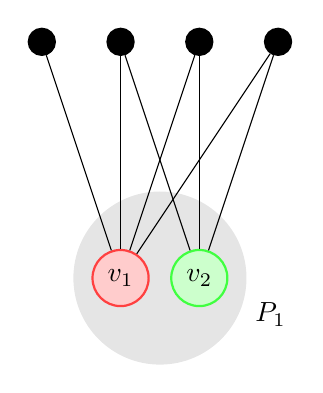
\begin{tikzpicture} 
		[includer/.style= {minimum size=3mm,thick,circle,draw=red!75,fill=red!20}, 
		included/.style= {minimum size=3mm,thick,circle,draw=green!75,fill=green!20}, 
		other/.style= {minimum size=3mm,thick,circle,draw=black,fill=black}, 
		transition/.style={thick,draw=black,fill=black!20}] 
		
		\node[other] (n3) at ( -1,3) {}; 
		\node[other] (n4) at ( 0,3) {}; 
		\node[other] (n5) at ( 1,3) {}; 
		\node[other] (n6) at ( 2,3) {}; 
		
		\node[includer] (n1) at ( 0,0) {$v_1$}
			edge [-]	(n3)
			edge [-]	(n4)
			edge [-]	(n5)
			edge [-]	(n6)
		;
		
		\node[included] (n2) at ( 1,0) {$v_2$}
			edge [-]	(n4)
			edge [-]	(n5)
			edge [-]	(n6)
		;
		
	
		\begin{pgfonlayer}{background} 
			\node [fill=black!10,circle,fit=(n1) (n2),label=350:$P_1$] {}; 
		\end{pgfonlayer} 
		
	\end{tikzpicture} 
\caption{Neighbourhood inclusion example: node $v_1$ will be removed from the graph as its neighbourhood completely contains $N(v_2)$.}
	\label{fig:neighbourinclusion}
\end{figure}
	
	\item{A lower bound for the chromatic number of the graph is obtained by finding a maximal clique in the partitions graph $G'$. Finding a clique of size $\omega$ in $G'$ implies that at least $\omega$ different colors are needed for coloring the partitions graph, and the same lower bound clearly holds for $G$. All partitions in the clique will have their colors fixed to $1,\ldots,\omega$ in order to reduce the number of possible colorings, since each of them must be painted using a different color.}
	\item{As in step 2, partitions that contain at least one node with degree less than the lower bound found in the previous step are removed. A node with strictly less than $\omega$ neighbours can be assigned a color among $1,\ldots,\omega$, knowing that no color conflicts will occur; and since there are already $\omega$ colors required, the chromatic number is not increased by that assignment, and therefore the node can be discarded.}
\end{enumerate}

Last 3 steps are performed until no more changes are made to the graph. The resulting largest clique found is used to fix the colors of the partitions included in it. 

Every step is processed by brute force, since their running time is polynomial in the size of the graph, except for step 4 for which we use the algorithm presented below.

\subsubsection*{Partitions graph clique detection}

To find the maximum clique in the partitions graph we use a simple backtracking algorithm. Since the running time of this algorithm can be excessive for a preprocessing step, we bound the running time of this algorithm to five seconds; however, the algorithm usually ends much sooner, as the partitions graph is not only smaller but also much less dense than the original graph. 

In case the time bound is reached, the best solution found so far is returned. As the backtracking uses DFS to explore all possible solutions, a reasonably good solution is generated early in the algorithm, therefore a valid result is obtained regardless its interruption.

Starting with an initial node, the algorithm keeps a list of valid candidates for the clique, which is updated on each iteration by removing all nodes that are not adjacent to the clique. Keeping both the candidates list and all adjacency lists sorted by degree makes computing the intersection between these lists faster, and produces better initial solutions that can be used to prune other solutions later.

\begin{algorithm}
\caption{Finding a maximum clique in a simple graph $G=<V,E>$}
\label{alg:gpclique}

\begin{algorithmic}

\STATE sort all nodes and adjacency lists descendingly by degree

\FORALL{initial node $v$ in $V$}
	\STATE initialize \textit{clique} with node $v$
	\STATE initialize \textit{candidates} with $N(v)$
	\CALL clique 
\ENDFOR

\PROC{clique}
	\IF{\textit{candidates} is empty}
		\STATE update \textit{best} solution if current \textit{clique} is better
	\ELSIF{\textit{clique}.size + \textit{candidates}.size $\leq$ \textit{best}.size}
		\STATE prune current tree
	\ELSE
		\STATE pop node $u$ from \textit{candidates} and add it to \textit{clique}
		\STATE intersect \textit{candidates} with $N(u)$ and store \textit{removed} nodes
		\CALL clique
		\STATE remove node $u$ from \textit{clique}
		\STATE add \textit{removed} nodes back to \textit{candidates} 
		\CALL clique
	\ENDIF
\ENDPROC

\end{algorithmic}
\end{algorithm} 

\subsection{Initial heuristic}

A good initial heuristic solution gives an upper bound on the solution, eliminates a large number of variables and restrictions in the model, and can be used as an initial incumbent solution for the branch and cut algorithm. 

In order to generate this solution, we use the modification of the \textsc{dsatur} algorithm for partitioned graphs presented in \ref{sec:heur}. Since the algorithm generates an implicit enumeration of all possible colorings, which might take too long to compute, its running time is bounded to five seconds. The coloring of the partitions in the clique $K$ is fixed to labels $1, \ldots, \omega$ in order to reduce the solutions set.

\subsection{Initialization}

Using the initial solution as an upper bound $\hat{\chi}$ for the chromatic number, it is possible to eliminate all $x_{ij}$ and $w_j$ variables with $j > \hat{\chi}$, thus greatly reducing the number of involved variables and restrictions in the model.

Another optimization is to fix the colors for all partitions involved in the clique $K$ found during the preprocessing stage. Since it is not possible to determine which node within the partition is to be colored, we simply set to zero all $x_{ij}$ variables for nodes within the partitions that use a different color than the one assigned. Formally, let $K = \{ P_{K_1}, \ldots, P_{K_\omega} \}$ be the initial clique, then:
\begin{align*}
x_{ij} = 0 \quad &\forall i \in K[l],\ \forall 1 \leq l \leq \omega,\ \forall j \neq l \\
w_j = 1 \quad &\forall 1 \leq j \leq \omega
\end{align*}

Also, in case the partition being fixed to a color $j_k$ has a single node in it, then variable $x_{ij_0}$, where $i$ is the single node in the partition, is fixed to $1$.

Another bound based on nodes degree is imposed. A node $v$ of partition degree $\delta_P(v)$ can always be colored with a label $j_k$ such that $1 \leq j_k \leq \delta_P(v) + 1$, since it will be neighbour to at most $\delta_P(v)$ different colors, therefore any set of $\delta_P(v) + 1$ colors contains at least one valid label that does not generate color conflicts.  
\begin{equation*}
x_{ij} = 0 \quad \forall i \in V,\ \forall 1 \leq j \leq \delta_P(v) + 1 \\
\end{equation*}

Finally, in case minimum partition index breaking symmetry restrictions (\ref{eqn:minlabel}) are being used, this is, the color with the lowest label is assigned to the color class containing the partition with the lowest index, another bound can be imposed on $x_ij$ variables. Since in the worst case all partitions will have a different color, then a partition with index $k$ will never be colored with label greater than $k$. Therefore, the following bound is imposed:
\begin{equation*}
x_{ij} = 0 \quad \forall P_k \in P,\ \forall i \in P_k,\ \forall j > k \\
\end{equation*}

\subsection{Cuts separation}

For each family of valid inequalities listed in \ref{sec:ineqs}, an heuristic is implemented to find a set of valid inequalities being violated in a given linear relaxation of the model. Note that in most cases, finding all violated inequalities in a solution is NP, so heuristic procedures must be applied. 

Since these algorithms are applied frequently during the branch and cut tree, it is imperative that their running time is as fast as possible, in order to minimize the added overhead to the whole algorithm.

\subsubsection*{Extended clique cuts}

Separation of extended clique cuts (\ref{ineq:extendedclique}) is done using a very similar algorithm to \ref{alg:gpclique}, adapted to partitioned graphs and without backtracking, so running time is acceptable for a separation algorithm. This algorithm is executed once for each color, and nodes are sorted based not on their degree but on their $x_{ij}$ value in the current solution.

For each initial node, a clique is constructed until the corresponding inequality is broken, and extended to up to $\kappa$ maximal cliques using backtracking, making use of the \textit{candidates} collection (note that in this case, \textit{candidates} is initialized with not only the initial node's neighbours, but also with all the nodes in its partition). In case no clique breaking the inequality is found, the next initial node is picked.

In order to avoid exploring the same solution space multiple times for different initial nodes, restrictions on how many times a node or an edge can be visited are applied. The resulting algorithm is presented in \ref{alg:sep:extclique}.

\begin{algorithm}
\label{alg:sep:extclique}

\begin{algorithmic}

\FORALL{color $j$ such that $w_j \geq \mu$}
\STATE sort all nodes and adjacency lists descendingly by $x_{ij}$ value
 
\FORALL{initial node $v$ in $V$}
	\STATE initialize \textit{clique} with node $v$
	\STATE initialize \textit{candidates} with $N(v) \cup P(v)$

	\WHILE{\textit{candidates} is not empty}
		\IF{current clique breaks inequality}
			\FORALL{maximal cliques $K$ containing \textit{clique} up to $\kappa$}
				\STATE add extended clique cut using $K$ and color $j$ 
			\ENDFOR
			\CONTINUE with next initial node
		\ELSIF{next candidate $u$ can be used}
			\STATE add $u$ to \textit{clique} and remove it from \textit{candidates} 
			\STATE remove nodes not adjacent to $u$ from \textit{candidates} 
		\ELSE
			\STATE remove $u$ from \textit{candidates}
		\ENDIF
	\ENDWHILE
		
\ENDFOR
\ENDFOR

\caption{Separation algorithm for extended clique cuts}

\end{algorithmic}
\end{algorithm} 

\subsubsection*{Component independent set inequalities}

Component hole \ref{ineq:chole} and component path \ref{ineq:cpath} inequalities are separated within the same procedure using a greedy heuristic. In a similar fashion to algorithm \ref{alg:sep:extclique}, for every color the graph is sorted according to $x_{ij}$ values, and for each initial node a component path or hole is greedily constructed. Once again, bounds for a maximum number of visits on each node are imposed, thus rejecting nodes with a certain number of visits or belonging to a partition already in the path, since this would violate the \textit{component} property.

On every iteration the most promising node is added to the path being built. In case this node is adjacent to a node already in the path (thus generating a hole), it is added only if it violates the corresponding inequality, otherwise, the next candidate is picked, and so forth. Algorithm \ref{alg:sep:ciset} resumes this process.

\begin{algorithm}
\label{alg:sep:ciset}

\begin{algorithmic}

\FORALL{color $j$ such that $w_j \geq \mu$}
\STATE sort all nodes and adjacency lists descendingly by $x_{ij}$ value
 
\FORALL{initial node $v$ in $V$}
	\STATE initialize \textit{path} with node $v$

	\LOOP
		\FORALL{valid node $u$ adjacent to last node in the path}
			\IF{$u$ is adjacent to a previous node $w$ in the path}
				\IF{hole $H=[u,\ldots,w]$ violates inequality \ref{ineq:chole}}
					\STATE add component hole inequality with hole $H$ and color $j$
					\CONTINUE with next initial node
				\ENDIF
			\ELSE
				\STATE add node $u$ to \textit{path}	
				\IF{current \textit{path} breaks inequality \ref{ineq:cpath}}
					\STATE add component path inequality with \textit{path} and color $j$
					\CONTINUE with next initial node
				\ENDIF
			\ENDIF
		\ENDFOR
	\ENDLOOP
\ENDFOR

\ENDFOR

\caption{Separation algorithm for component independent set cuts}

\end{algorithmic}
\end{algorithm}

As an alternative to the previous algorithm, we also implemented the hole detection algorithm presented in \cite{nikolopoulos2004hole}. We adapted the algorithm presented in the paper to reject a node if it belongs to a partition already in the path, therefore exploring only component holes; and tested this implementation against the previous one in section \ref{sec:results}.

\subsubsection*{Partitions graph independent set inequalities}

For both path and hole inequalities (\ref{ineq:gpiset}) over the partitions graph $G'$, algorithms equivalent to the ones used for component independent sets are applied as separation heuristics.

Graph $G'$ is constructed once at the beginning of the branch and cut and is then used as input for these heuristics. Since there are no $x_{ij}$ variables to use for sorting the nodes of the graph, the value $\sum_{i \in P_k} x_{ij}$ is used for each partition $P_k$, this is, the sum of the values of the partition's nodes.

\subsubsection*{Block color inequalities}

Block color inequalities (\ref{ineq:blockcp}) are explored using brute force, since there are no more than $c \times q$ of them, and checking whether they are violated or not can be performed fast enough.

Alternatively, they can be added initially to the cut pool provided by the branch and cut framework, instead of manually checking them at each cuts iteration.

\subsection{Node selection strategies}

On each iteration of the branch and cut algorithm, an unprocessed node must be chosen to be solved. Determining which node will be handled next is known as the \textit{node selection} strategy.

There are different standard node selection strategies, all of them implemented by the branch-and-cut framework we used. In section \ref{sec:results} we experiment with the behaviour of the algorithm under different strategies:
\begin{itemize}
	\defitem{DFS}{Depth-first search, picks the last node opened, attempting to generate an integral solution by diving to the bottom of the tree as fast as possible. This strategy has low memory consumption as relatively few nodes are left unprocessed on every iteration.}
	\defitem{BFS}{Breadth-first search, picks the first node opened; this strategy solves every open node with at the same depth before proceeding to the following depth level. It usually has memory issues, as a large number of nodes tend to be left open, thus making this a poor choice in most cases.}
	\defitem{BestBound}{Best-bound, picks the open node with best objective function available, thus closer to an integer feasible solution. This strategy usually reports the best results.}
	\defitem{BestEstimate}{Best-estimate uses \textit{an estimate of a given node's progress toward integer feasibility relative to its degradation of the objective function}\cite{cplex121}; it improves the chance of finding feasible solutions when they are difficult to generate, which is not the case in \PCP{}.}
\end{itemize}


\subsection{Branching strategies}
\label{subsec:alg:branching}

After each node in the branch and cut tree is processed, new child nodes are created by subdividing the problem into two easier subproblems; this is usually done by \textit{branching} on a certain variable. Usually, in the case of binary variables, a variable $x$ with a fractional value in the relaxation is chosen, and the two subproblems are created by fixing $x = 0$ and $x = 1$ and re-processing. Alternatively, bounds on expressions, instead of on variables, can be set.

\begin{figure}[h]
	\label{fig:branching}
	\centering
	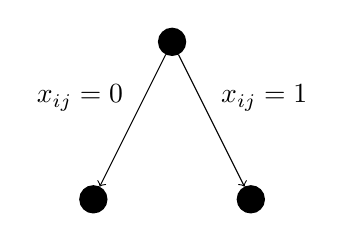
\begin{tikzpicture} 
		[black/.style= {minimum size=3mm,thick,circle,draw=black,fill=black},
		 branch/.style= {->}] 
		
		\node[black] (n1) at ( 0,0) {};
		\node[black] (n2) at ( 2,0) {};
		
		\node[black] (n3) at ( 1,2) {}
			edge[branch] node[swap,auto] {$x_{ij} = 0$} (n1)
			edge[branch] node[auto] {$x_{ij} = 1$} (n2)	
		;
		
	\end{tikzpicture} 
\end{figure}

Whichever method of branching is chosen, it requires that the solutions represented by the union of all subproblems cover all integral solutions represented by the parent node; otherwise, feasible solutions may be left unexplored.

Choosing which variable to branch on, and what bounds are implied within each branch, is part of what is called the branching strategy. 

\subsubsection*{Static priorities}

The simplest way to choose which variable to branch on is to assign a priority to each $x_{ij}$, which will be used to pick the branching variable when necessary: the integer infeasible variable with the highest priority is picked on every branching. 

We experimented in section \ref{subsec:resultsbranching} with combinations of the following criteria for selecting variable $x_{ij}$:

\begin{itemize}
\item{The number of partitions adjacent to node $i$}
\item{The size of the partition containing node $i$}
\item{The label of color $j$}
\end{itemize}

Using this criteria has the huge drawback that no information regarding the actual value of the $x_{ij}$ variable is used, so these priorities work best as a tie-breaker for another strategy.

\subsubsection*{Fractional values}
\label{subsubsec:alg:branch:frac}

A common practice is to pick the most fractional variable to branch on. We determine such variable as:
\[
\min_{x_{ij}} \{ |x_{ij} - 0.5| \}
\]

In case of a tie, we use the static priority set for the variables to determine which one use to branch on. We also experimented in section \ref{subsec:resultsbranching} with the opposite criteria, this is, branching on the less fractional value (excluding those variables with already integral values).

This is a common branching technique, but does not exploit any particular feature of the problem being studied, unlike the one described below.

\subsubsection*{Degree of saturation}
\label{subsubsec:alg:branch:dsatur}

A branching strategy specifically related to the partitioned coloring problem is to branch on a node with the highest degree of saturation. Since these nodes are usually the most difficult ones to handle, it is reasonable to fix their values as early as possible in the branch and cut tree.

This criteria for picking the branching variable requires first to compute an approximate degree of saturation for every node and choosing the one with the largest value, $i^*$, in order to obtain a set of candidate variables $x_{i^*j_0}, x_{i^*j_1}, \ldots, x_{i^*j_c}$ (once again, ties between nodes are broken using the already defined priorities).

Since the only available values are those of the fractional solution, we color one node in each partition using the largest value within the partition and neighbours: this is, for every node $i$ and color $j$ combination, if the value $x_{ij}$ is larger than all of its neighbours and nodes in the same partition, as well as larger than an arbitrary lower bound ($0.7$)\footnote{Note that if the classic constraints are being used, \ref{eqn:partsum} and \ref{eqn:adjscolorp}, by specifying a lower bound higher than $0.5$ it is not necessary to verify that the node has the highest value among its neighbours or within the partition, as it will be assured by the restrictions; the check is required in case alternative restrictions are used, such as allowing more than one node to be colored or grouping multiple color conflicts into single constraints.}, we assign color $j$ to node $i$. Note that some partitions might be left uncolored, in this case they will not contribute to the degree of saturation of their neighbours.

\begin{equation}
\label{eqn:fixcriteria}
v_i \leftarrow j \text{ if } x_{ij} > 0.7 \wedge x_{ij} > x_{kj}\ \forall k \in N(i) \cup P(i)
\end{equation}

\begin{nuevo}
Having chosen a node $v_i$ for branching, we must choose which variable $x_{i^*j^*}$ from the set of candidate $x_{i^*j_0}, x_{i^*j_1}, \ldots, x_{i^*j_c}$ will be branched on. We have implemented two different strategies for this:
\begin{itemize}
	\item{Choose the variable $x_{i^*j^*}$ with the highest value from the set, and branch on $x_{i^*j^*} = 0$ and $x_{i^*j^*} = 1$; this results in a classic $0-1$ branching on the variable corresponding to the most saturated node with its most \textit{likely} color.}
	\item{Create up to $C+1$ subproblems, one for each possible coloring of the node, branching on $x_{i^*j_0} = 1, \ldots, x_{i^*j_c} = 1$, plus another child which sets all $x_{i^*j_0}$ variables to zero, in case the node is not colored within its partition.}
\end{itemize}
\end{nuevo}

\sout{
From the mentioned set of candidates $x_{i^*j_0}, x_{i^*j_1}, \ldots, x_{i^*j_c}$, the variable with the highest value is chosen for branching. Overall, we are branching on the node with the highest degree of saturation, fixing it to the most probable color it was assigned in the relaxation.
}

\subsubsection*{Implied bounds}
\label{subsubsec:alg:branch:bounds}

When manually specifying the branching variable and creating the subproblems, it is also possible to fix more variables that would be affected by the value assigned to the first one.

Regardless of the branching variable, it is possible to fix all color variables $w_j$ to $1$ for $j = 1,\ldots,\ceil{z}$, where $z$ is the value of the objective function of the current node's relaxation. For example, if the sum of all $w_j$ variables is $5.3$, which is a lower bound on the chromatic number, we can be sure that at least $6$ different colors are needed to color the graph, and therefore all $w_1,\ldots,w_6$ can be set to $1$.

When branching down on the selected variable\footnote{Fixing the branch variable's value to 0.}, there are no more logical implications than the previous one that can be used to bound more variables. This is easy to see since setting an $x_{ij}$ variable to zero implies that a certain color will not be used for a certain node, but does not grant any information on which \textit{node} on the partition will be colored and with which \textit{color}.

Branching up, on the other hand, provides much more information. Whenever a variable $x_{i^*j^*}$ is set to $1$, this is, node $i^*$ in partition $P(i^*)$ is assigned color $j^*$, we may specify the following conditions for that branch:

\begin{itemize}
\item Every other color-node combination in partition $P(i^*)$ can be set to zero, as only one node must be assigned a color in the partition.
\[
x_{ij} = 0 \quad \forall i \in P(i^*),\ \forall j \in C,\ i \neq i^* \vee j \neq j^*
\]

\item Every node adjacent to $i^*$ cannot use color $j^*$ in order to avoid color conflicts.
\[
x_{ij^*} = 0 \quad \forall i \in N(i^*)
\]
\end{itemize}

\subsection{Primal heuristic}
\label{subsec:alg:primal}

The algorithm used to create an integer feasible solution from the relaxation's solution is called the \textit{primal heuristic}. A typical primal heuristic consists in rounding the values of every fractional variable to the nearest integer value, as long as this process satisfies all the restrictions imposed by the model.

For \PCP{} we implemented a primal heuristic based on the \textsc{dsatur} algorithm. Given a fractional solution $x^*$, for every variable $x_{ij}$ with a large enough value, we fix that node-color combination. The criteria used for determining when a variable is fixed is the same as the one depicted in \ref{eqn:fixcriteria}.

Also, for every variable $x_{ij}$ with an upper bound set to $0$ as a product of the branching in the branch and cut tree, we forbid that node-color combination.

Having all these values fixed, an extremely short run of \textsc{dsatur} is executed, bounded to 200 milliseconds. The algorithm works reasonably fast as more and more variables are fixed, and bounds for the optimal coloring can be inferred from the branch and cut tree, further shortening the exploration of possible solutions. 
\begin{itemize}
\item{Value $\ceil{\sum_{j \in C} w_j}$ of the node's relaxation is a lower bound to the integer solution, so in case \textsc{dsatur} finds a solution using that number of colors, it can be assured that it is the local optimum.}
\item{The solution of the primal heuristic will be used as the global upper bound, replacing the current incumbent solution, only if it uses less colors. Therefore, \textsc{dsatur} is bounded to exploring solutions that use strictly less colors than the incumbent.}
\end{itemize}

The best coloring obtained by the algorithm is then used as an incumbent solution for the node. In case certain symmetry breaking restrictions are in place, a reordering of the labels assigned to each color class might have to be performed.

\subsection{Implicit enumeration}
\label{subsec:alg:implicit}

Early experimentation with the branch and cut algorithm and with the \textsc{dsatur} algorithm has shown that, for relatively small instances, the latter explores all possible solutions much faster than the former, since it does not have all the overhead imposed by the different artifacts present in a full branch and cut.

Therefore, when we have reduced the problem size to a relatively small one by fixing node-color assignments during the branching process, instead of proceeding with the traditional branch and cut algorithm, we execute a full run of \textsc{dsatur}. Since most partitions are already colored, the number of possible solutions is reasonably small to be fully explored.

In section \ref{sec:results} we experiment with different values for the number of uncolored partitions in the branch and cut tree to be used as the threshold for stopping the branch and cut and starting an unbounded execution of \textsc{dsatur}.

\subsection{Implementation details}

The branch and cut algorithm was implemented in Java 1.6 using CPLEX version 12.1 both as a branch-and-cut framework and a linear programming solver for relaxations. 

We made use of branch, heuristic and cut callbacks provided by the CPLEX API to manage the branching strategy, inject primal solutions and apply custom cuts on both the root and internal nodes.
\begin{itemize}
\item{The branch callback is invoked once the processing of a certain node has been completed in order to determine how to create the child subproblems; inside this callback we implement the different dynamic branching strategies described in \ref{subsec:alg:branching}. Static priorities are fixed during the initialization of the problem. This callback is also used to prune the branch and cut tree once a certain number of partitions have been fixed in order to proceed with the implicit enumeration from \ref{subsec:alg:implicit}.}
\item{The heuristic callback is invoked after the linear relaxation of a node has been solved, and provides the fractional values from the relaxation's solution to derive an integral feasible solution, using the color degree strategy explained in \ref{subsec:alg:primal}. We make use of this callback to inject the integral solution derived from implicit enumeration (\ref{subsec:alg:implicit}).}
\item{The cut callback is invoked after the linear relaxation is solved; every certain number of nodes the separation heuristics are invoked in an attempt to add planes to cut off the current linear solution. After the cuts are added, the relaxation is solved again, and more iterations of cutting planes may be optionally executed; while few iterations are performed in the internal nodes, a larger number is executed in the root.}
\end{itemize} 

The framework was configured to use standard branch and cut search, instead of dynamic search, to correctly determine the performance of the developed strategies. Multi-core processing was also disabled.

%!TEX root = pcp.tex

\section{Computational results}
\label{sec:results}

This section contains all the results obtained from the computational experiments executed. We devised a test suite for each algorithm or strategy to parametrize, and picked the configuration with the best results for each subsequent test. Tested components include the model formulation, \textsc{dsatur} strategy, branch criteria, primal heuristic, separation algorithms, etc.

\subsubsection*{Testing environment}

We executed all tests on a \TODO{computer, JVM and OS description}.

\subsubsection*{Graphs instances}

We used different types of instances on each test depending on the focus of the test itself. Overall, we used mostly random graphs, as well as certain \textsc{dimacs} challenge instances\cite{dimacs} for our last tests. In the case of random graphs, we used multiple instances (between three and five, depending on running times) for each parameterization and reported the average results.  

Random graphs were built according to two different schemes:
\begin{itemize}
	\defitem{Erdos-R\'enyi}{Also known as binomial graphs\cite{erdosrenyi}, each of the possible edges between the set of $n$ nodes is chosen to be included with probability $p$; this parameter determines the density of the graph. This procedure generates graphs with an equal distribution of degrees among its nodes.
	\begin{figure}
	  \begin{center}
	    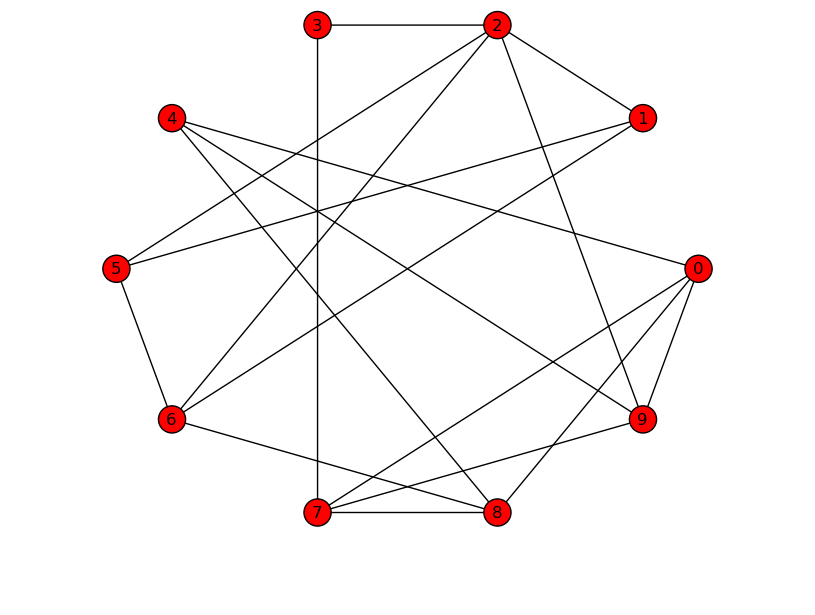
\includegraphics[scale=0.5]{imgs/binomial-10-04.png}
	  \end{center}
		\label{results:graph:binomial}
		\caption{Sample random binomial graph with $10$ nodes and a $40\%$ probability to create an edge between each pair of nodes.}
	\end{figure}
	}
	\defitem{Holme-Kim}{Also known as powerlaw cluster graphs\cite{holme2002growing}, the graph is constructed iteratively by attaching each new node to a number $t$ of already existing nodes using preferential attachment based on the degree of existing nodes. Also, after the addition of each edge, there is a probability $p$ that a triangle will be created by adding an additional edge. These graphs are controlled by two parameters: node count $n$ and density $p$; value $t$ is inferred as the product between $p$ and $n$.
	\begin{figure}
	  \begin{center}
	    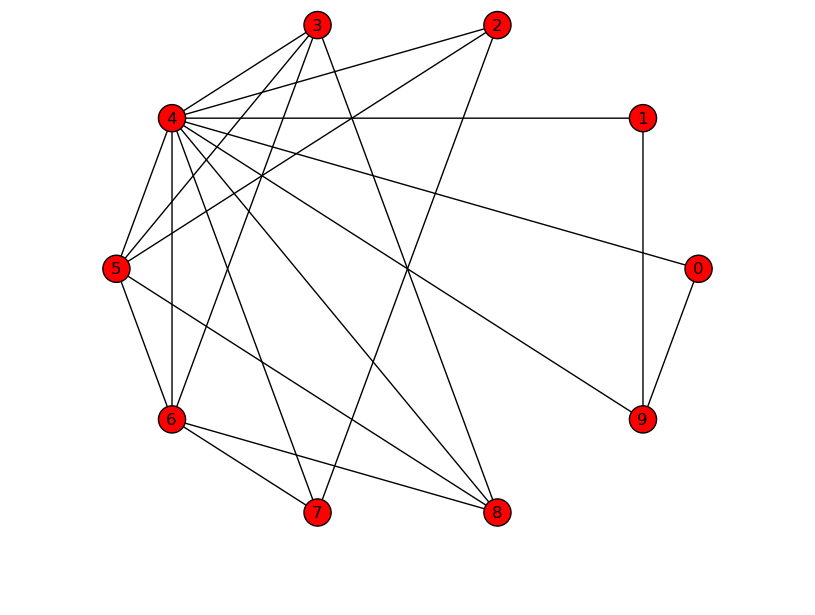
\includegraphics[scale=0.5]{imgs/hk-10-04.png}
	  \end{center}
		\label{results:graph:binomial}
		\caption{Sample random powerlaw cluster graph with $10$ nodes, note how certain nodes have a much higher degree than the others.}
	\end{figure}
	} 
\end{itemize}

Since both of the previous procedures generate unpartitioned graphs, they are partitioned after their generation by grouping nodes with consecutive indices in partitions of a certain size. For most instances we used a fixed partition size of $2$, although in some cases we used random sizes varying from $1$ to $4$.

These random graphs were generated using the \textit{NetworkX} python package\cite{networkx}, version $1.1$.
%!TEX root = pcp.tex

\subsection{Models comparison}

We executed a test suite for determining which inequalities to use in the formulation of the problem. Recall from section \ref{sec:model} that there are several restrictions that can be applied to define the model, as well as additional ones that may strengthen the model or reduce the number of symmetrical solutions.

In order to test the effectiveness of the different formulations, we applied a fixed number of cutting planes iterations, using all implemented cuts with a slightly aggressive configuration, and reported the resulting MIP gap and running time (in seconds), as well as how many rounds of cutting planes were executed. It is worth noting that in some cases fewer iterations than total were applied as the separation heuristics were not able to find any more violated inequalities.

For these tests we used binomial graphs with a fixed size of 100 nodes with exactly 2 nodes per partition, and powerlaw cluster graphs with the same size, changing only the density of the graphs. All graphs were preprocessed beforehand.

\subsubsection{Adjacency constraints}

We first tested the four different adjacency (or color conflict) constraints we had proposed, using arbitrarily chosen constraints \ref{eqn:partsum}, \ref{eqn:lowerlabel} and \ref{eqn:wjleqsumcolor} to complete the model:

\begin{align*}
&\sum_{i \in P_k} \sum_{j \in C} x_{ij} = 1 &\quad \forall P_k \in P \tag{\ref{eqn:partsum}} \\
&w_j \geq w_{j+1} &\quad \forall 1 \leq j < c \tag{\ref{eqn:lowerlabel}} \\
&w_j \leq \sum_{i \in V} x_{ij} &\quad \forall j \in C \tag{\ref{eqn:wjleqsumcolor}} \\
\end{align*}

The different adjacency constraints being tested in this experiment are the following: 

\begin{align*}
&x_{ij} + x_{kj} \leq w_j \sumheight &\quad \forall (i,k) \in E, \; \forall j \in C \tag{\ref{eqn:adjscolorp}} \\
&x_{ij} + x_{kj} \leq 1 \sumheight &\quad \forall (i,k) \in E, \; \forall j \in C \tag{\ref{eqn:adjscolorpone}} \\
&\sum_{i \in N(i_0)} x_{i_0j} + r * x_{i_0j} \leq r * w_j &\quad \forall j \in C, \; \forall i_0 \in V \tag{\ref{eqn:adjsneighb}} \\
&\sum_{i \in P_k \cap N(i_0)} x_{ij} + x_{i_0j} \leq w_j &\quad \forall j \in C, \; \forall P_k \in P, \; \forall i_0 \in V \tag{\ref{eqn:adjsperpart}} 
\end{align*}

Results are displayed on table \ref{table:modelsadj}. Differences between gaps are almost non existent, whereas time required changes greatly between graphs with different densities. On higher density graphs, constraints \ref{eqn:adjsneighb} using a clique coverage of the neighbourhood report a better running time than the others; while on lower density \ref{eqn:adjscolorpone} works better than \ref{eqn:adjscolorp}, even though the former uses $n \dot c$ additional constraints \ref{eqn:nodelessthanwj}.

Graphics \ref{fig:models:adj} show the evolution of the gap for four particular representative instances, one for each of the evaluated densities in binomial graphs. Gap evolution is very similar among different configurations, except for \ref{eqn:adjsneighb} which is remarkably slower to achieve the same gap in low density graphs. At $40\%$ and $60\%$ densities, \ref{eqn:adjscolorpone} not only works better than \ref{eqn:adjscolorp} as reported in table \ref{table:modelsadj}, but also achieves the same gap slightly faster.

\begin{sidewaystable}
\centering

	\begin{tabular}{|c|ccc|ccc|ccc|ccc|}
	\hline
	\multicolumn{1}{|c|}{Id} & \multicolumn{3}{|c|}{Constraint \ref{eqn:adjscolorp}} & \multicolumn{3}{|c|}{Constraint \ref{eqn:adjscolorpone}} & \multicolumn{3}{|c|}{Constraint \ref{eqn:adjsneighb}} & \multicolumn{3}{|c|}{Constraint \ref{eqn:adjsperpart}} 
	\\
	& gap & rounds & time & gap & rounds & time & gap & rounds & time & gap & rounds & time 
	\\
	\hline
	EW 20\% & 0.458 & 14.6 & 5.632 & 0.458 & 10.6 & \b{4.568} & 0.458 & 20.4 & 7.915 & 0.458 & 16.2 & 5.728
	\\
	EW 40\% & 0.466 & 22.4 & 16.998 & 0.466 & 25.6 & \b{14.09} & 0.466 & 32.6 & 17.884 & 0.466 & 24.8 & 16.976
	\\
	EW 60\% & 0.42 & 62.8 & 98.642 & 0.42 & 57.4 & \b{77.694} & 0.42 & 72.6 & 87.575 & 0.42 & 78.6 & 120.138
	\\
	EW 80\% & 0.292 & 193.0 & 449.054 & 0.296 & 181.2 & 469.844 & 0.292 & 192.4 & \b{349.557} & 0.294 & 160.0 & 451.126
	\\
	\hline
	HK 10\% &  0.2 &  0.8 & 0.156 &  0.2 &  0.8 & 0.128 &  0.2 &  0.8 & 0.106 &  0.2 &  0.8 & 0.168
	\\
	HK 20\% & 0.12 &  0.6 & 0.278 & 0.12 &  0.6 & 0.324 &  0.2 &  1.0 & 0.181 & 0.12 &  0.6 & 0.306
	\\
	HK 30\% &  0.0 &  0.8 & 0.308 &  0.0 &  0.8 & 0.276 &  0.0 &  3.2 & 0.489 &  0.0 &  0.8 & 0.318
	\\
	HK 40\% & 0.048 &  2.2 & 0.28 & 0.048 &  3.0 & 0.312 & 0.048 &  5.2 & 0.416 & 0.048 &  2.6 & 0.292
	\\
	\hline 
	 \end{tabular}
	
	\caption{Comparison of different color conflict constraints on the model formulation: adjacent nodes sum bounded by $w_j$ (\ref{eqn:adjscolorp}), adjacent nodes sum bounded by $1$ (\ref{eqn:adjscolorpone}), adjacencies grouped by partition (\ref{eqn:adjsperpart}) and using clique coverage of the neighbourhood (\ref{eqn:adjsneighb}).}
	\label{table:modelsadj}
\end{sidewaystable}


\begin{figure}
\centering
\subfloat[EW 100 Nodes 20\% Density]{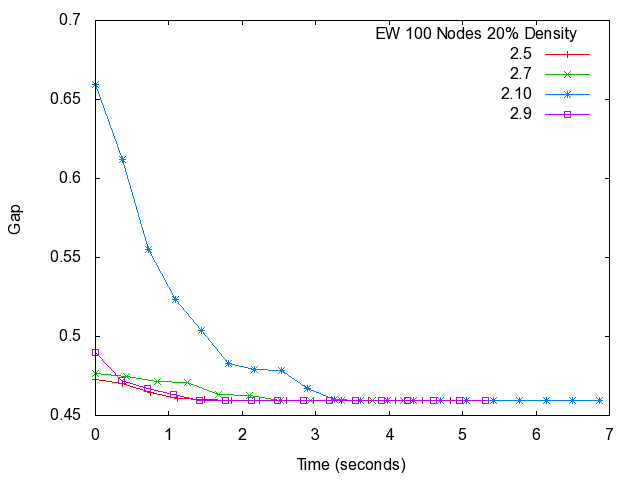
\includegraphics[width=0.6\textwidth]{plots/modelsgap-ew20-n100-adj.png}}
\subfloat[EW 100 Nodes 40\% Density]{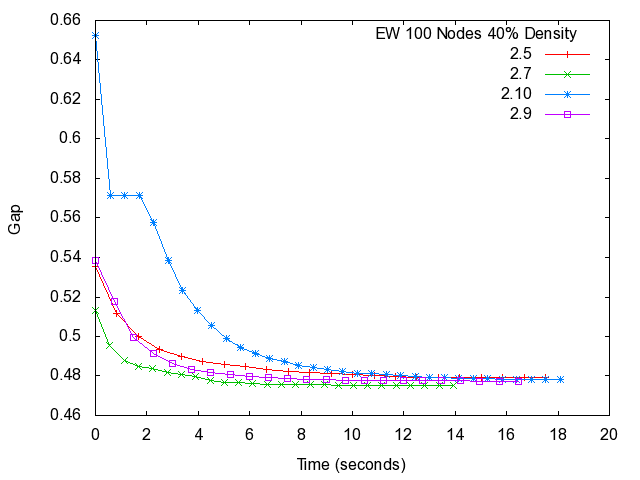
\includegraphics[width=0.6\textwidth]{plots/modelsgap-ew40-n100-adj.png}}
\\
\subfloat[EW 100 Nodes 60\% Density]{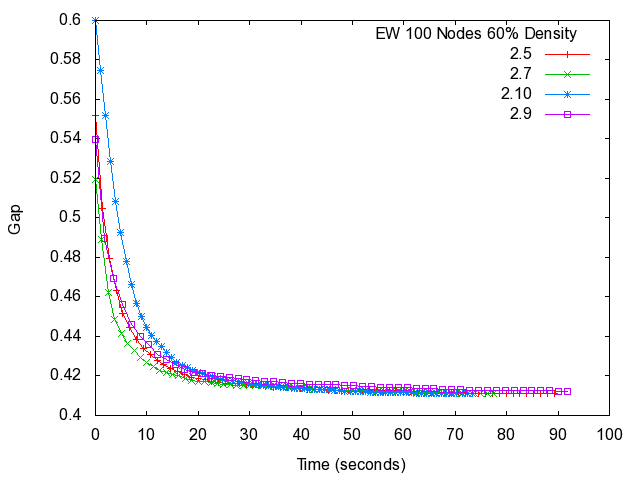
\includegraphics[width=0.6\textwidth]{plots/modelsgap-ew60-n100-adj.png}}
\subfloat[EW 100 Nodes 80\% Density]{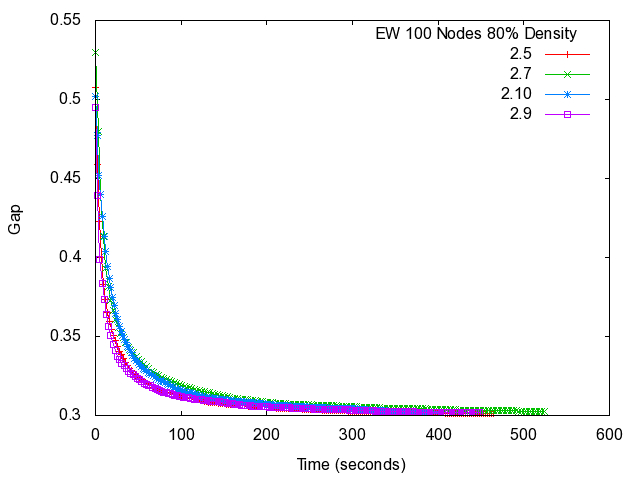
\includegraphics[width=0.6\textwidth]{plots/modelsgap-ew80-n100-adj.png}}
\caption{Comparison of the inclusion of different color conflict constraints in the model, visualizing evolution of the gap during time in a cutting planes algorithm. Compared constraints are: adjacent nodes sum bounded by $w_j$ (\ref{eqn:adjscolorp}), adjacent nodes sum bounded by $1$ (\ref{eqn:adjscolorpone}), adjacencies grouped by partition (\ref{eqn:adjsperpart}) and using clique coverage of the neighbourhood (\ref{eqn:adjsneighb}).}
\label{fig:models:adj}
\end{figure}

\subsubsection{Colored nodes per partition}

A quick test we also ran in parallel was to determine whether to paint exactly one node per partition (\ref{eqn:partsum}), or to relax this constraint and allow for painting more than a single node (\ref{eqn:partsumgeq}). 

\begin{table}
\centering

\begin{tabular}{|c|cc|cc|}
\hline
\multicolumn{1}{|c|}{Id} & \multicolumn{2}{|c|}{At least 1} & \multicolumn{2}{|c|}{Exactly 1}
\\
 & gap & time & gap & time
\\
\hline
EW 20\% & 0.46 & 5.472 & 0.458 & 7.915
\\
EW 40\% & 0.466 & 17.324 & 0.466 & 17.884
\\
EW 60\% & 0.42 & 93.578 & 0.42 & 87.575
\\
EW 80\% & 0.294 & 354.612 & 0.292 & 349.557
\\
\hline
HK 10\% &  0.2 & 0.112 &  0.2 & 0.106
\\
HK 20\% &  0.2 & 0.136 &  0.2 & 0.181
\\
HK 30\% &  0.0 & 0.434 &  0.0 & 0.489
\\
HK 40\% & 0.076 & 0.398 & 0.048 & 0.416
\\
\hline 
 \end{tabular}

\caption{Comparison of constraints specifying whether exactly one node must be assigned one color in the partition, or at least one node should be painted with at least one color.}
\label{table:models:partsum}
\end{table}

Results on table \ref{table:models:partsum} confirm our expectations: while the former has a slightly larger running time, it also reports a slightly lower gap than the latter in some cases. The simplicity provided by \ref{eqn:partsum} when extracting solutions from the model (when constructing the the partial solutions to be processed during the primal heuristic, or during the branching process) makes us choose this option in our formulation.

\subsubsection{Model strengthening}

We also compared applying only constraint \ref{eqn:wjleqsumcolor}, which ensures that variable $w_j$ is set only if a node uses color $j$ (regardless of the objective function), to adding restrictions \ref{eqn:wjgeqsumnode} and \ref{eqn:wjgeqsumpart}:

\begin{align*}
\sum_{j \in C} w_j \geq \sum_{j \in C} j x_{ij} \quad \forall i \in V \tag{\ref{eqn:wjgeqsumnode}} \\
\sum_{j \in C} w_j \geq \sum_{j \in C} \sum_{i \in P_k} j x_{ij} \quad \forall P_k \in P \tag{\ref{eqn:wjgeqsumpart}}
\end{align*}

\begin{table}
\centering

\begin{tabular}{|c|ccc|ccc|ccc|}
\hline
\multicolumn{1}{|c|}{Id} & \multicolumn{3}{|c|}{\ref{eqn:wjleqsumcolor}} & \multicolumn{3}{|c|}{\ref{eqn:wjgeqsumnode}} & \multicolumn{3}{|c|}{\ref{eqn:wjgeqsumpart}}
\\
 & gap & niters & time & gap & niters & time & gap & niters & time
\\
\hline
EW 20\% & 0.458 & 20.4 & 7.915 & 0.458 & 15.8 & 7.318 & 0.458 & 15.4 & \b{7.286}
\\
EW 40\% & 0.466 & 32.6 & 17.884 & 0.466 & 37.6 & 19.464 & 0.466 & 32.0 & \b{17.748}
\\
EW 60\% & 0.42 & 72.6 & \b{87.575} & 0.42 & 84.2 & 91.272 & 0.42 & 79.4 & 89.03
\\
EW 80\% & 0.292 & 192.4 & \b{349.557} & 0.294 & 170.0 & 355.518 & 0.294 & 180.6 & 378.936
\\
\hline
HK 10\% &  0.2 &  0.8 & \b{0.106} &  0.2 &  0.8 & 0.108 &  0.2 &  0.8 & 0.112
\\
HK 20\% &  0.2 &  1.0 & \b{0.181} &  0.2 &  1.0 & 0.198 &  0.2 &  1.0 & 0.184
\\
HK 30\% &  0.0 &  3.2 & \b{0.489} &  0.0 &  3.2 & 0.552 &  0.0 &  3.2 & 0.51
\\
HK 40\% & 0.048 &  5.2 & \b{0.416} & 0.048 &  4.0 & 0.398 & 0.048 &  5.2 & 0.438
\\
\hline 
 \end{tabular}

\caption{Comparison of different model strengthening constraints: (\ref{eqn:wjleqsumcolor}) which ensures that variable $w_j$ is set only if a node uses color $j$, and (\ref{eqn:wjgeqsumnode}) and (\ref{eqn:wjgeqsumpart}) which eliminate certain fractional constraints, adding over all colors of node and of a partition, respectively.}

\label{table:models:colorbound}

\end{table}

\begin{figure}
\centering
\subfloat[EW 100 Nodes 20\% Density]{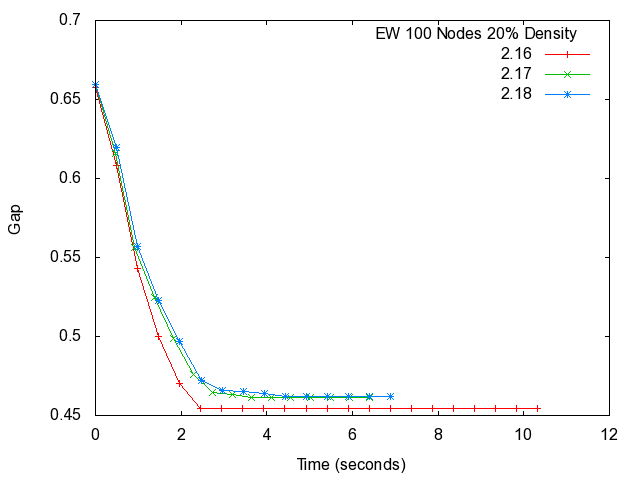
\includegraphics[width=0.6\textwidth]{plots/modelsgap-ew20-n100-cb.png}}
\subfloat[EW 100 Nodes 40\% Density]{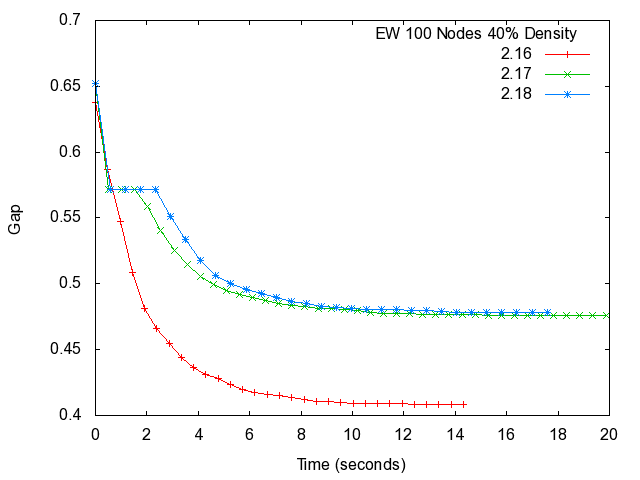
\includegraphics[width=0.6\textwidth]{plots/modelsgap-ew40-n100-cb.png}}
\\
\subfloat[EW 100 Nodes 60\% Density]{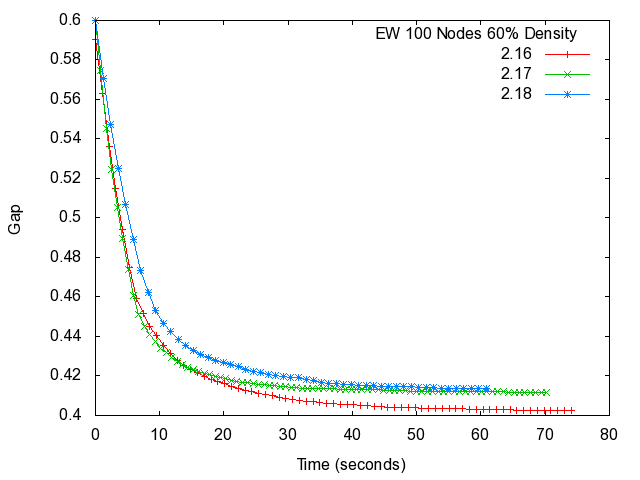
\includegraphics[width=0.6\textwidth]{plots/modelsgap-ew60-n100-cb.png}}
\subfloat[EW 100 Nodes 80\% Density]{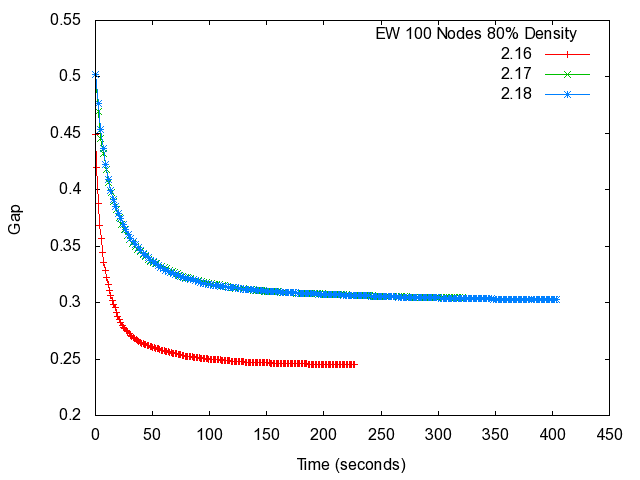
\includegraphics[width=0.6\textwidth]{plots/modelsgap-ew80-n100-cb.png}}
\caption{Comparison of the inclusion of model strengthening constraints in the model, visualizing evolution of the gap during time in a cutting planes algorithm. Compared constraints are: (\ref{eqn:wjleqsumcolor}) which ensures that variable $w_j$ is set only if a node uses color $j$, and (\ref{eqn:wjgeqsumnode}) and (\ref{eqn:wjgeqsumpart}) which eliminate certain fractional constraints, adding over all colors of node and of a partition, respectively.}
\label{fig:models:colorbound}
\end{figure}

Results on table \ref{table:models:colorbound} show that there is very little difference between the three variants. Overall, the simplest one, \ref{eqn:wjleqsumcolor}, seems to be the fastest one to execute, although taking slightly more cuts iterations in non-medium density graphs. 

The graphics \ref{fig:models:colorbound} present, as before, the evolution of the gap for these different configurations on a representative binomial instance for each tested density. Configuration \ref{eqn:wjleqsumcolor} is shown to be not only the one returning the best gap (even for very little difference with the others), but also the fastest one.

\subsubsection{Symmetry breaking}

Results obtained from comparing no symmetry breaking constraints whatsoever with color label (\ref{eqn:lowerlabel}), node count (\ref{eqn:symnodecount}) and minimum node label (\ref{eqn:nodeszero},\ref{eqn:minlabel}) ordering restrictions are shown on table \ref{table:models:sym}. The evolution of the obtained gap in time for different densities is shown in figure \ref{fig:models:sym}.

\begin{align*}
& w_j \geq w_{j+1} \sumheight \quad &\forall 1 \leq j < c \tag{\ref{eqn:lowerlabel}} \\
& \sum_{i \in V} x_{ij} \geq \sum_{i \in V} x_{ij+1} \quad &\forall 1 \leq j < c \tag{\ref{eqn:symnodecount}} \\
& x_{ij} = 0 \sumheight \quad &\forall j > p(i) + 1 \tag{\ref{eqn:nodeszero}} \\
& x_{ij} \leq \sum_{l = j-1}^{k-1} \sum_{u \in P_l} x_{uj-1} \quad &\forall 1 < k \leq q, \; \forall i \in P_k, \; \forall 1 < j \leq k \tag{\ref{eqn:minlabel}}
\end{align*}

It is with these constraints that significative changes in solution gaps are found. While there is little difference between applying or not the simplest restrictions \ref{eqn:lowerlabel} (although they are required for the validity of other inequalities and bounds), stricter restrictions that further eliminate symmetrical solutions report much lower gaps, in some cases even reaching optimality at this stage. 

Minimum partition index constraints (\ref{eqn:nodeszero},\ref{eqn:minlabel}) have the best gaps, require fewer cutting planes iterations, and run within acceptable times (in some cases even faster than its counterparts). The graphics in \ref{fig:models:sym} support this, showing that \ref{eqn:minlabel} either reaches a better gap faster than the others, or simply returns a better gap when solving the first relaxation (without obtaining a big improvement when applying cutting planes).

\begin{sidewaystable}

\centering

\begin{tabular}{|c|ccc|ccc|ccc|ccc|}
\hline
\multicolumn{1}{|c|}{Id} & \multicolumn{3}{|c|}{Constraint \ref{eqn:minlabel}} & \multicolumn{3}{|c|}{None} & \multicolumn{3}{|c|}{Constraint \ref{eqn:lowerlabel}} & \multicolumn{3}{|c|}{Constraint \ref{eqn:symnodecount}}
\\
 & gap & niters & time & gap & niters & time & gap & niters & time & gap & niters & time
\\
\hline
EW 20\% & 0.46 & 20.8 & 3.086 & \b{0.458} & 18.2 & 8.45 & \b{0.458} & 20.4 & 7.915 & 0.466 & 16.0 & 6.032
\\
EW 40\% & \b{0.298} & 34.4 & 20.342 & 0.466 & 31.6 & 21.244 & 0.466 & 32.6 & 17.884 & 0.314 & 39.8 & 31.484
\\
EW 60\% & \b{0.04} & 34.8 & 153.702 & 0.42 & 73.2 & 96.82 & 0.42 & 72.6 & 87.575 & 0.16 & 86.4 & 433.19
\\
EW 80\% & \b{0.052} & 43.2 & 299.66 & 0.294 & 192.2 & 401.3 & 0.292 & 192.4 & 349.557 & 0.16 & 100.6 & 202.282
\\
\hline
HK 10\% &  \b{0.2} &  0.6 & 0.082 & 0.206 &  4.4 & 0.26 &  \b{0.2} &  0.8 & 0.106 & 0.15 &  0.6 & 0.084
\\
HK 20\% & \b{0.12} &  0.6 & 0.144 & 0.206 &  9.8 & 0.752 &  0.2 &  1.0 & 0.181 & \b{0.12} &  0.6 & 0.12
\\
HK 30\% &  0.0 &  2.0 & 0.314 &  0.0 &  3.4 & 0.516 &  0.0 &  3.2 & 0.489 &  0.0 &  2.4 & 0.454
\\
HK 40\% & 0.048 &  3.8 & 0.316 & 0.05 &  6.2 & 0.494 & 0.048 &  5.2 & 0.416 & \b{0.024} &  4.4 & 0.376
\\
\hline 
 \end{tabular}

\caption{Comparison of the inclusion of different symmetry breaking constraints in the model: assigning the lowest color label to the color class with the lowest node index \eqref{eqn:minlabel}, applying no constraint whatsoever, forcing lower labels to be used first \eqref{eqn:lowerlabel} and assigning the lowest color label to the color class with the greatest number of nodes \eqref{eqn:symnodecount}.}
\label{table:models:sym}

\end{sidewaystable}

\begin{figure}
\centering
\subfloat[EW 100 Nodes 20\% Density]{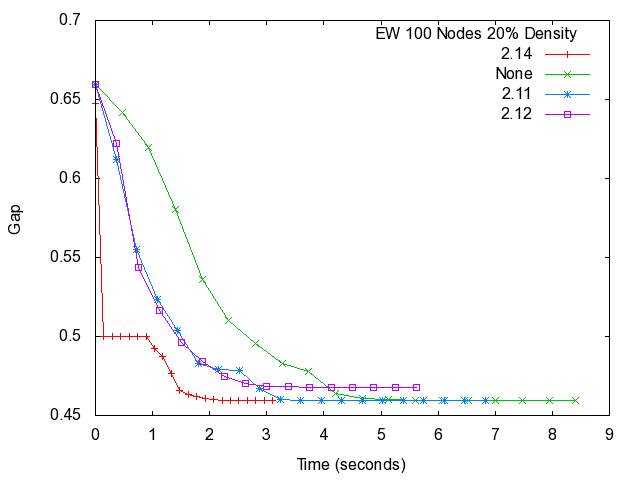
\includegraphics[width=0.6\textwidth]{plots/modelsgap-ew20-n100-sym.png}}
\subfloat[EW 100 Nodes 40\% Density]{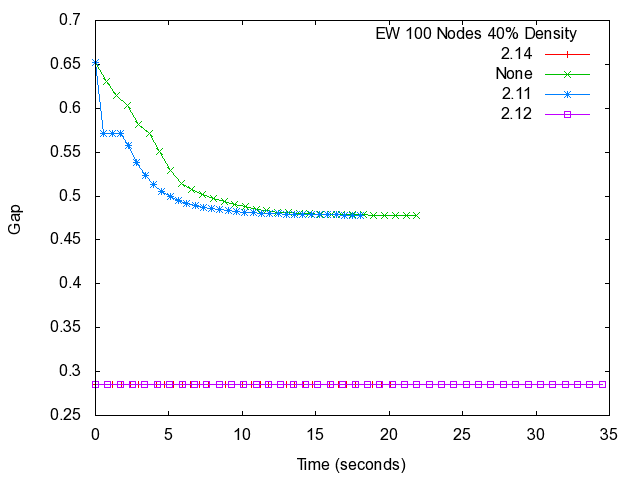
\includegraphics[width=0.6\textwidth]{plots/modelsgap-ew40-n100-sym.png}}
\\
\subfloat[EW 100 Nodes 60\% Density]{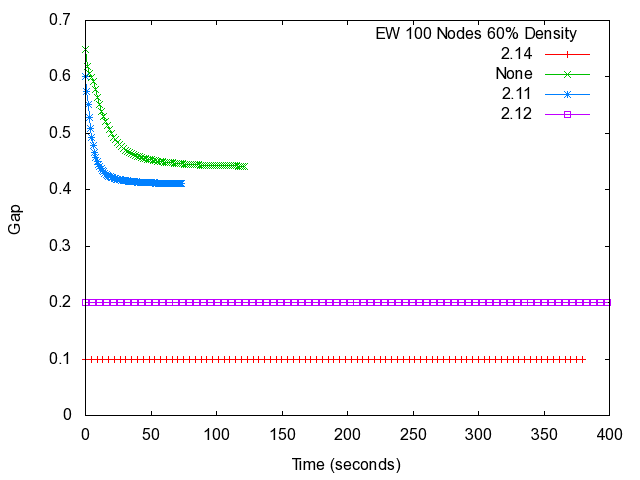
\includegraphics[width=0.6\textwidth]{plots/modelsgap-ew60-n100-sym.png}}
\subfloat[EW 100 Nodes 80\% Density]{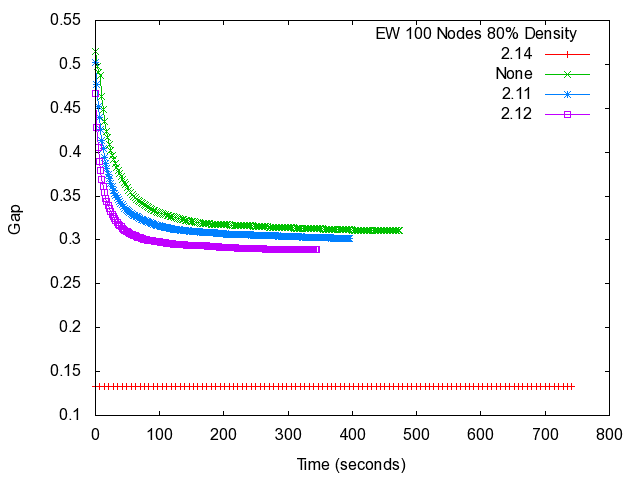
\includegraphics[width=0.6\textwidth]{plots/modelsgap-ew80-n100-sym.png}}
\caption{Comparison of the inclusion of different symmetry breaking constraints in the model, visualizing evolution of the gap during time in a cutting planes algorithm. Compared constraints are: assigning the lowest color label to the color class with the lowest node index \eqref{eqn:minlabel}, applying no constraint whatsoever, forcing lower labels to be used first \eqref{eqn:lowerlabel} and assigning the lowest color label to the color class with the greatest number of nodes \eqref{eqn:symnodecount}.}
\label{fig:models:sym}
\end{figure}


\subsubsection{Chosen formulation from cutting planes}
\label{subsubsec:results:model:chosen}

Taking into account all previous results in a cutting planes algorithm, the set of constraints that we will use in the \PCP{} formulation for subsequent computational experiments will be the following:

\begin{align}
\sum_{i \in P_k} \sum_{j \in C} x_{ij} = 1 \quad &\forall P_k \in P \tag{\ref{eqn:partsum}} \\
 \sum_{i \in N(i_0)} x_{i_0j} + r * x_{i_0j} \leq r * w_j \quad &\forall j \in C, \; \forall i_0 \in V \tag{\ref{eqn:adjsneighb}} \\
 w_j \leq \sum_{i \in V} x_{ij} \quad &\forall j \in C \tag{\ref{eqn:wjleqsumcolor}} \\
 x_{ij} \leq \sum_{l = j-1}^{k-1} \sum_{u \in P_l} x_{uj-1} \quad &\forall 1 < k \leq q, \; \forall i \in P_k, \; \forall 1 < j \leq k \tag{\ref{eqn:minlabel}} \\
 %w_j \geq w_{j+1} \sumheight \quad &\forall 1 \leq j < c \tag{\ref{eqn:lowerlabel}} \\
  x_{ij}, w_{j} \in \{0,1\} \quad &\forall i \in V, \; \forall j \in C \sumheight \nonumber
\end{align}

First two constraints define the problem itself, by specifying that a node must be colored in each partition and no color conflicts must occur; constraints \ref{eqn:wjleqsumcolor} simply strengthen the linear relaxation; and \ref{eqn:minlabel} eliminate symmetrical solutions. Last set of constraints are the binary restrictions.

Note that while adjacency restrictions \ref{eqn:adjscolorpone} reported better results than the chosen ones (\ref{eqn:adjsneighb}) in most cases, the latter worked better in dense graphs, which are the ones that, due to a larger problem size, take longer to solve their linear relaxation. Therefore, we opt for improving the resolution of the hardest graphs instead of getting slightly better results in the rest. 

\subsubsection{Branch and bound testing}

While the previous formulation was chosen for working on a cutting planes algorithm, we are also interested in the behaviour of different models in standard branch and bound algorithms. 

We tested many variations to the chosen model in a branch and bound algorithm, bound to $1800$ seconds, with graphs with $90$ nodes, partition size $2$ and different densities. The branch and bound uses default \textsc{cplex} settings, no custom callbacks were yet applied.

\begin{table}
\label{table:models:bnb}
\centering

\begin{tabular}{|c|c|c|c|c|c|c|c|}
\hline
\multicolumn{1}{|c|}{Id} & \multicolumn{1}{|c|}{C1} & \multicolumn{1}{|c|}{C2} & \multicolumn{1}{|c|}{C3}  & \multicolumn{1}{|c|}{C4} & \multicolumn{1}{|c|}{C5} & \multicolumn{1}{|c|}{C6} & \multicolumn{1}{|c|}{C7} 
\\
\hline
EW 20 N=90 & \textbf{0.00} & \textbf{0.00} & 0.25  & \textbf{0.00} & 0.43 & 0.25 & 0.25
\\
EW 40 N=90 & 0.33 & \textbf{0.22} & 0.33 & 0.33 & 0.33 & 0.28 & 0.35
\\
EW 60 N=90 & 0.39 & 0.37 & 0.41 & 0.37 & 0.48 & \textbf{0.15} & 0.38
\\
EW 80 N=90 & 0.38 & 0.43 & 0.31 & 0.39 & 0.41 & \textbf{0.10} & 0.38
\\
\hline 
 \end{tabular}

\caption{Gap obtained in a standard branch and bound algorithm for different models.}

\end{table}

We present in table \ref{table:models:bnb60} the following configurations, chosen based on their results:

\begin{itemize}
\defitem{C1}{Chosen model from cutting planes experimentation phase.} %S4
\defitem{C2}{Relaxes that exactly one node must be painted per partition (\ref{eqn:partsum}) by replacing it with at least one painted per partition (\ref{eqn:partsumgeq}).} %S1
\defitem{C3}{Uses simple color conflict constraints, requiring that two adjacent nodes cannot use the same color (\ref{eqn:adjscolorpone}).} %S3
\defitem{C4}{Strengthens the model using not only \ref{eqn:wjleqsumcolor} restrictions but also applying \ref{eqn:wjgeqsumpart}.} %S8
\defitem{C5}{Uses no symmetry breaking constraints whatsoever.} %S9
\defitem{C6}{Bases symmetry breaking on the number of nodes of each color class (\ref{eqn:symnodecount}).} %S10
\defitem{C7}{Applies constraints \ref{eqn:adjsperpart} for color conflict.} %S11
\end{itemize}

Results were most interesting. The formulation chosen for the cutting planes algorithm yielded good results only for lowest density graphs. In other cases, using different models returned better results:
\begin{itemize}
\item In graphs with $40\%$ density, relaxing the \ref{eqn:partsum} constraint on painting one node per partition greatly reduces the obtained gap, as can be seen in the results for $C2$.
\item In the most dense graphs, varying the strategy for color conflicts to use constraint \ref{eqn:symnodecount} yields much better results.
\end{itemize}

Considering the results returned by using constraint \ref{eqn:symnodecount}, we re-tested all of the previous configurations changing the default symmetry breaking strategy from \ref{eqn:minlabel} to \ref{eqn:symnodecount}, except for C1 which kept the original settings. This time, we executed a branch and bound algorithm on much smaller graphs (60 nodes), restricting ourselves to 10-minute runs and \textbf{not} providing the algorithm with any initial solution, in order to obtain zero gap and compare running times.

\begin{table}
\centering

\begin{tabular}{|c|c|c|}
\hline
\textit{Strategy} & {$40\%$} & {$60\%$}
\\
\hline
C1 & 17.41 & 151.12
\\
C2 & 15.42 & 55.51
\\
C4 & 4.47 & 30.30
\\
C3 & \textbf{0.37} & 30.06
\\
C6 & 4.48 & 30.50
\\
C5 & \textbf{0.78} & 56.68
\\
C7 & 51.47 & \textbf{15.22}
\\
\hline 
 \end{tabular}

\caption{Running time until resolution obtained in a standard branch and bound algorithm for different models, in binomial graphs with 60 nodes, without providing an initial heuristic solution.}
\label{table:models:bnb60}

\end{table}

The most interesting results are found in $40\%$ and $60\%$ density graphs, and are displayed in table \ref{table:models:bnb60}. It is also worth noting that C7 was the only one to solve all $80\%$ density graphs to optimality.

This time, using a simpler model, both regarding color conflict and symmetry breaking, yielded very good results in low density graphs. In higher densities, applying constraints \ref{eqn:adjsperpart} for color conflicts produces excellent results, which is surprising as the efectiveness of these constraints was highly related to partition sizes, not densities.

\spacedhrule
Throughout this chapter we have tested a significant number of different models, which were obtained by combining different constraints, and tested them in different scenarios by using different algorithms. Results changed greatly between those scenarios.

Although we will be using the formulation devised in \ref{subsubsec:results:model:chosen} for testing other settings throughout the following experimentations, we will reuse all the results exposed here as alternative models for the final branch and cut algorithm, in order to pick the best performing model for the final version of the algorithm.

\clearpage
%!TEX root = pcp.tex

\subsection{Partitioned \textsc{dsatur}}
\label{subsec:resultspdsatur}

Considering we had three different partitioned \textsc{dsatur} implementations (see section \ref{subsec:heur:pdsatur}), we ran quick tests on multiple graphs to determine how they performed when executed for short periods of time. For each instance, we executed the different algorithms for one minute, and report the lowest bound for the chromatic number obtained, as well as how fast was this bound obtained. Since we will be using \textsc{dsatur} mostly as an heuristic, it is of our interest that good solutions are found as quickly as possible.

\subsubsection*{Hardest partition parametrization}

Before comparing the three different algorithms, we had to fix the criteria used to pick the \textit{hardest partition} on each call in this variant of the algorithm\footnote{Recall that this strategy picked the hardest partition on each call, and then the easiest node from it.}. As we had already mentioned, the criteria used is a combination of:

\begin{itemize}
	\item{Color degree of the partition, defined as the number of different colors adjacent to all of the nodes in the partition; considering that a larger color degree implies a harder partition to color}
	\item{Size of the partition, as a larger partition being colored earlier helps reducing the problem size, therefore the larger the partition the earlier it should be handled}
	\item{Number of uncolored partitions adjacent to the partition, equivalent to the tie breaking criteria used for classic \textsc{dsatur}} 
\end{itemize}

We generated six different configurations, based on all different possible orderings of these items. For example, for the first configuration, we first compared by the number of adjacent uncolored partitions, then by the degree of saturation, and finally by the size of the partition. The following are the configurations we established:

\begin{itemize}
\defitem{C1}{Uncolored, saturation, size}
\defitem{C2}{Saturation, uncolored, size}
\defitem{C3}{Uncolored, size, saturation}
\defitem{C4}{Saturation, size, uncolored}
\defitem{C5}{Size, uncolored, saturation}
\defitem{C6}{Size, saturation, uncolored}
\end{itemize}

Results in table \ref{table:pdsatur:hardp} show little difference for most instances in which partition size is constant (fixed to two nodes). Whereas in some cases, mostly those with lower density, configurations C1, C3 and C5 (those who choose the hardest partition by number of uncolored neighbour partitions before by saturation degree) find the solution earlier, in other cases configurations C2, C4 and C6 report better times. All of them find always nearly the same values for the chromatic number.

Differences arise, however, when we have different partition sizes. Configurations C1 and C3, those who pick the partition on uncolored neighbours, obtain better bounds in less time than the others. Surprisingly, configurations based on partition sizes offer the worst results for these cases.

Since we will be working mostly with partitioned graphs with equal partition sizes, we will not take into consideration configurations that use this as a criteria; and as graphs with higher density have been taking the longest time to process, we will prefer a configuration that best deals with this cases, such as C2.

\begin{sidewaystable}
\label{table:pdsatur:hardp}
\centering

\begin{tabular}{|c|cc|cc|cc|cc|cc|cc|}
\hline
\multicolumn{1}{|c|}{Graphs} & \multicolumn{2}{|c|}{C1} & \multicolumn{2}{|c|}{C2} & \multicolumn{2}{|c|}{C3} & \multicolumn{2}{|c|}{C4} & \multicolumn{2}{|c|}{C5} & \multicolumn{2}{|c|}{C6}
\\
 & chi & found & chi & found & chi & found & chi & found & chi & found & chi & found
\\
\hline
EW 20\% N=140 &  6.0 & 0.192 &  5.8 & 1.514 &  6.0 & 0.196 &  5.8 & 1.504 &  6.0 & 0.184 &  5.8 &  1.5
\\
EW 40\% N=140 & 10.0 & 6.372 &  9.6 & 16.878 & 10.0 & 6.384 &  9.6 & 16.874 & 10.0 & 6.382 &  9.6 & 16.886
\\
EW 60\% N=140 & 14.2 & 27.692 & 14.4 & 16.208 & 14.2 & 27.758 & 14.4 & 16.154 & 14.2 & 27.79 & 14.4 & 16.184
\\
EW 80\% N=140 & 21.8 & 8.29 & 21.8 & 8.138 & 21.8 & 8.314 & 21.8 & 8.14 & 21.8 & 8.294 & 21.8 & 8.148
\\
\hline
EW 50\% N=140 P=(1..2) & 16.2 & 1.414 & 16.0 & 5.232 & 16.2 & 1.414 & 15.6 & 0.428 & 18.0 & 19.652 & 15.6 & 0.612
\\
EW 50\% N=140 P=(1..3) & 10.4 & 6.61 & 11.4 & 11.576 & 10.4 & 6.648 & 12.4 &  9.7 & 13.0 & 1.17 & 12.6 & 0.068
\\
EW 50\% N=140 P=(1..4) &  9.2 & 6.788 &  9.4 & 10.542 &  9.2 & 6.794 & 10.8 & 5.37 & 11.0 & 30.262 & 10.8 & 14.542
\\
EW 50\% N=140 P=(2..3) &  8.8 & 3.366 &  8.8 & 0.486 &  8.8 & 3.35 &  9.8 & 0.37 &  9.6 & 6.964 &  9.8 & 0.382
\\
EW 50\% N=140 P=(2..4) &  7.2 & 0.366 &  7.2 & 16.604 &  7.2 & 0.36 &  8.2 & 20.728 &  8.8 & 0.15 &  8.2 & 25.316
\\
EW 50\% N=140 P=(3..4) &  6.6 & 1.504 &  6.6 & 4.122 &  6.6 & 1.506 &  6.6 & 0.23 &  6.6 & 0.246 &  6.6 & 0.23
\\
\hline
EW 50\% N=080 &  7.0 & 2.248 &  7.0 & 0.658 &  7.0 & 2.252 &  7.0 & 0.648 &  7.0 & 2.25 &  7.0 & 0.656
\\
EW 50\% N=100 &  8.2 & 19.472 &  8.0 & 10.01 &  8.2 & 19.504 &  8.0 & 10.008 &  8.2 & 19.526 &  8.0 & 10.014
\\
EW 50\% N=120 & 10.0 & 12.04 & 10.0 & 1.578 & 10.0 & 12.066 & 10.0 & 1.588 & 10.0 & 12.058 & 10.0 & 1.586
\\
EW 50\% N=140 & 11.6 & 8.88 & 11.8 & 3.832 & 11.6 & 8.892 & 11.8 & 3.81 & 11.6 & 8.904 & 11.8 & 3.826
\\
EW 50\% N=160 & 13.4 & 6.066 & 13.4 & 6.352 & 13.4 & 6.07 & 13.4 & 6.344 & 13.4 & 6.068 & 13.4 & 6.35
\\
EW 50\% N=180 & 14.0 & 1.376 & 14.0 & 6.962 & 14.0 & 1.382 & 14.0 & 6.97 & 14.0 & 1.382 & 14.0 & 6.92
\\
EW 50\% N=200 & 16.2 & 0.57 & 15.4 & 0.766 & 16.2 & 0.574 & 15.4 & 0.776 & 16.2 & 0.572 & 15.4 & 0.774
\\
\hline
HK 10\% N=140 &  6.4 & 0.106 &  6.4 & 0.02 &  6.4 & 0.106 &  6.4 & 0.02 &  6.4 & 0.114 &  6.4 & 0.02
\\
HK 20\% N=140 &  9.4 & 0.114 &  9.0 & 9.804 &  9.4 & 0.112 &  9.0 & 9.824 &  9.4 & 0.11 &  9.0 & 9.846
\\
HK 30\% N=140 & 12.4 & 3.066 & 11.8 & 20.746 & 12.4 & 3.066 & 11.8 & 20.758 & 12.4 & 3.066 & 11.8 & 20.818
\\
HK 40\% N=140 & 14.8 & 21.552 & 14.2 &  6.8 & 14.8 & 21.576 & 14.2 & 6.798 & 14.8 & 21.588 & 14.2 & 6.792
\\
\hline 
 \end{tabular}
\caption{Best value obtained for the chromatic number and time at which this value was obtained in one-minute runs of the \textit{hardest partition} version of \textsc{dsatur}, using different combinations of strategies to pick the hardest partition at each call.}

\end{sidewaystable}

\subsubsection*{Strategies comparison}

After fixing the \textit{hardest partition} strategy to C2, we will compare its performance with both the \textit{easiest node} and the \textit{randomized easiest node} variants. We ran the same tests as before, and present the results on table \ref{table:pdsatur:comp}.

Regardless of the configuration chosen for the \textit{hardest partition} variant, both \textit{easiest node} strategies find much better bounds within the one-minute running time. From those, the deterministic one offers slightly better results, and is therefore the algorithm that we will be using for the following experimentations. 

The randomized version might perform better in larger graphs on lengthier running periods, since it has a chance to find a different solution than the deterministic and obtain a sudden improvement on the bound, whereas the deterministic may spend several iterations trying similar assignments. However, in very short runs as these ones, the deterministic version is clearly preferred.  

\begin{table}
\label{table:pdsatur:comp}
\centering

\begin{tabular}{|c|cc|cc|cc|}
\hline
\multicolumn{1}{|c|}{Graphs} & \multicolumn{2}{|c|}{\textit{easiest node}} & \multicolumn{2}{|c|}{\textit{randomized node}} & \multicolumn{2}{|c|}{\textit{hardest partition}}
\\
 & chi & found & chi & found & chi & found
\\
\hline
EW 20\% N=140 &  5.0 & 0.004 &  5.0 & 0.016 &  5.8 & 1.514
\\
EW 40\% N=140 &  8.0 & 4.172 &  8.2 & 27.334 &  9.6 & 16.878
\\
EW 60\% N=140 & 12.4 & 10.062 & 12.4 & 4.656 & 14.4 & 16.208
\\
EW 80\% N=140 & 18.6 & 25.522 & 18.4 & 10.77 & 21.8 & 8.138
\\
\hline
EW 50\% N=140 P=(1..2) & 13.6 & 4.356 & 13.8 & 2.346 & 16.0 & 5.232
\\
EW 50\% N=140 P=(1..3) &  9.6 & 31.634 &  9.8 & 8.31 & 11.4 & 11.576
\\
EW 50\% N=140 P=(1..4) &  8.0 & 6.464 &  8.8 & 9.796 &  9.4 & 10.542
\\
EW 50\% N=140 P=(2..3) &  7.4 & 11.172 &  8.0 & 0.046 &  8.8 & 0.486
\\
EW 50\% N=140 P=(2..4) &  6.8 & 0.702 &  7.0 & 1.224 &  7.2 & 16.604
\\
EW 50\% N=140 P=(3..4) &  5.8 & 1.494 &  6.0 & 0.652 &  6.6 & 4.122
\\
\hline
EW 50\% N=080 &  6.0 & 2.584 &  6.4 & 0.778 &  7.0 & 0.658
\\
EW 50\% N=100 &  7.2 & 1.646 &  7.2 & 15.728 &  8.0 & 10.01
\\
EW 50\% N=120 &  9.0 & 0.042 &  9.0 & 1.618 & 10.0 & 1.578
\\
EW 50\% N=140 & 10.2 & 1.59 & 10.0 & 33.264 & 11.8 & 3.832
\\
EW 50\% N=160 & 11.2 & 5.134 & 11.8 & 2.576 & 13.4 & 6.352
\\
EW 50\% N=180 & 12.6 & 10.242 & 13.0 & 4.818 & 14.0 & 6.962
\\
EW 50\% N=200 & 13.6 & 14.636 & 14.0 & 0.966 & 15.4 & 0.766
\\
\hline
HK 10\% N=140 &  4.0 & 0.016 &  4.0 & 0.044 &  6.4 & 0.02
\\
HK 20\% N=140 &  6.0 & 0.016 &  6.0 & 0.168 &  9.0 & 9.804
\\
HK 30\% N=140 &  8.0 & 0.008 &  8.0 & 0.118 & 11.8 & 20.746
\\
HK 40\% N=140 &  9.8 & 0.002 &  9.8 & 0.008 & 14.2 &  6.8
\\
\hline 
 \end{tabular}

\caption{Best value obtained for the chromatic number and time at which this value was obtained in one-minute runs for the \textit{hardest partition}, \textit{easiest node} and \textit{randomized easiest node} versions of \textsc{dsatur}.}

\end{table}
%!TEX root = pcp.tex

\subsection{Branching strategies}
\label{subsec:resultsbranching}

\begin{itemize}
\item Static priorities: See branchstatic1, S4 wins, dont include tables
\item Dynamics: Compare fractional, dsatur, with and without color consec; both dsatur win, regardless consec color, gap found better, dont compare with gap
\item Bounds: Once dsatur is fixed, try with and without fixing bounds, see fixing works much better
\item Remark statics are faster than dynamics due to processing time
\end{itemize}

%!TEX root = pcp.tex

\chapter{Conclusions}
\label{sec:conclusions}

Conclusions...

\bibliographystyle{plain}
\bibliography{references}

\end{document}

